% small.tex
\documentclass[aspectratio=169]{beamer}
\usetheme{Boadilla}
\usepackage{amsmath}
\usepackage{graphicx}
\usepackage{wrapfig}
%algorithms and pseudo code
\usepackage{algorithm}
\usepackage[noend]{algpseudocode}
\usepackage{numprint}
\usepackage{subcaption}
\usepackage{media9}
\usepackage{bibentry}
\usepackage[autoplay,loop]{animate}
\usepackage[justification=centering]{caption}
\nobibliography*

\setbeamertemplate{bibliography item}[text]
\setbeamertemplate{author in head/foot}{\insertshortauthor}
\setbeamertemplate{navigation symbols}{}

\newcommand{\lenitem}[2][.6\linewidth]{\parbox[t]{#1}{\strut #2\strut}}
\newcommand{\outline}{
  \begin{frame}<beamer>
    \frametitle{Outline}
    \tableofcontents[currentsection]
  \end{frame}
}

\begin{document}

\title[Load Balancing on Many-Core and Accelerated Systems]{

Session 4: Heterogeneous Applications: \\
Maximizing Benefits While Minimizing Cost

\textbf{Load Balancing on Many-Core and Accelerated Systems}
}

\author[C. Smith]{\underline{Cameron W. Smith}, Gerrett Diamond, and Mark S. Shephard}

\institute[SCOREC]{
Scientific Computation Research Center \\
Rensselaer Polytechnic Institute
}

\date{April 25, 2019}


%----------- titlepage ----------------------------------------------%
\begin{frame}[plain]
  \titlepage
\end{frame}

%----------------------------------------------------------------------%
%----------- Systems --------------------------------------------------%
%----------------------------------------------------------------------%
\begin{frame}
  \frametitle{Load Balancing, Performance, and Scalability}
  \begin{itemize}
  \item Partitioning and Load Balancing - distributing work to maximize performance on a
  given machine
  \item Performance - time to solution
  \begin{itemize}
    \item local - serial, vectorized, threaded, or data parallel procedures on
      many-core processor or accelerator
    \item global - local operations + coordination/synchronization procedures
  \end{itemize}
  \item Scalability - efficiency with increase in computing power
    \begin{itemize}
    \item Weak - increase problem size with increase in computing power
    \item Strong - fixed problem size as computing power increases
    \end{itemize}
  \item High performance procedures are not necessarily
    scalable or portable (some parameter tuning, no algorithm changes
      required to get acceptable performance [1])
  \item Scalable procedures are not necessarily portable
  \end{itemize}
  \bigskip
  \small{[1] \url{https://performanceportability.org/perfport/definition/}}
\end{frame}

\section{Manycore and Accelerated Systems}
\begin{frame}
  \frametitle{Manycore and Accelerated Systems}
  \begin{columns}
    \begin{column}{0.7\textwidth}
      Manycore Node
      \begin{itemize}
        \item Many homogeneous cores provide all the computing power
        \item Each core can access filesystem and network
        \item Possibly multiple NUMA domains
      \end{itemize}
      Accelerated Node
      \begin{itemize}
        \item Host processor - dispatches accelerator work, facilitates
          communications, OS interactions
        \item Accelerator - provides most of the computing power \\
          e.g.) Summit GPUs have 95\% of memory bandwidth and 98\% of FLOPs
      \end{itemize}
      %Big-little
      %\begin{itemize}
      %  \item A few larger general purpose cores combined with smaller
      %    specialized cores, e.g.; DSP, network, sensing
      %  \item Enable and disable cores on the fly to save energy
      %\end{itemize}
    \end{column}
    \begin{column}{0.3\textwidth}
      \centering
      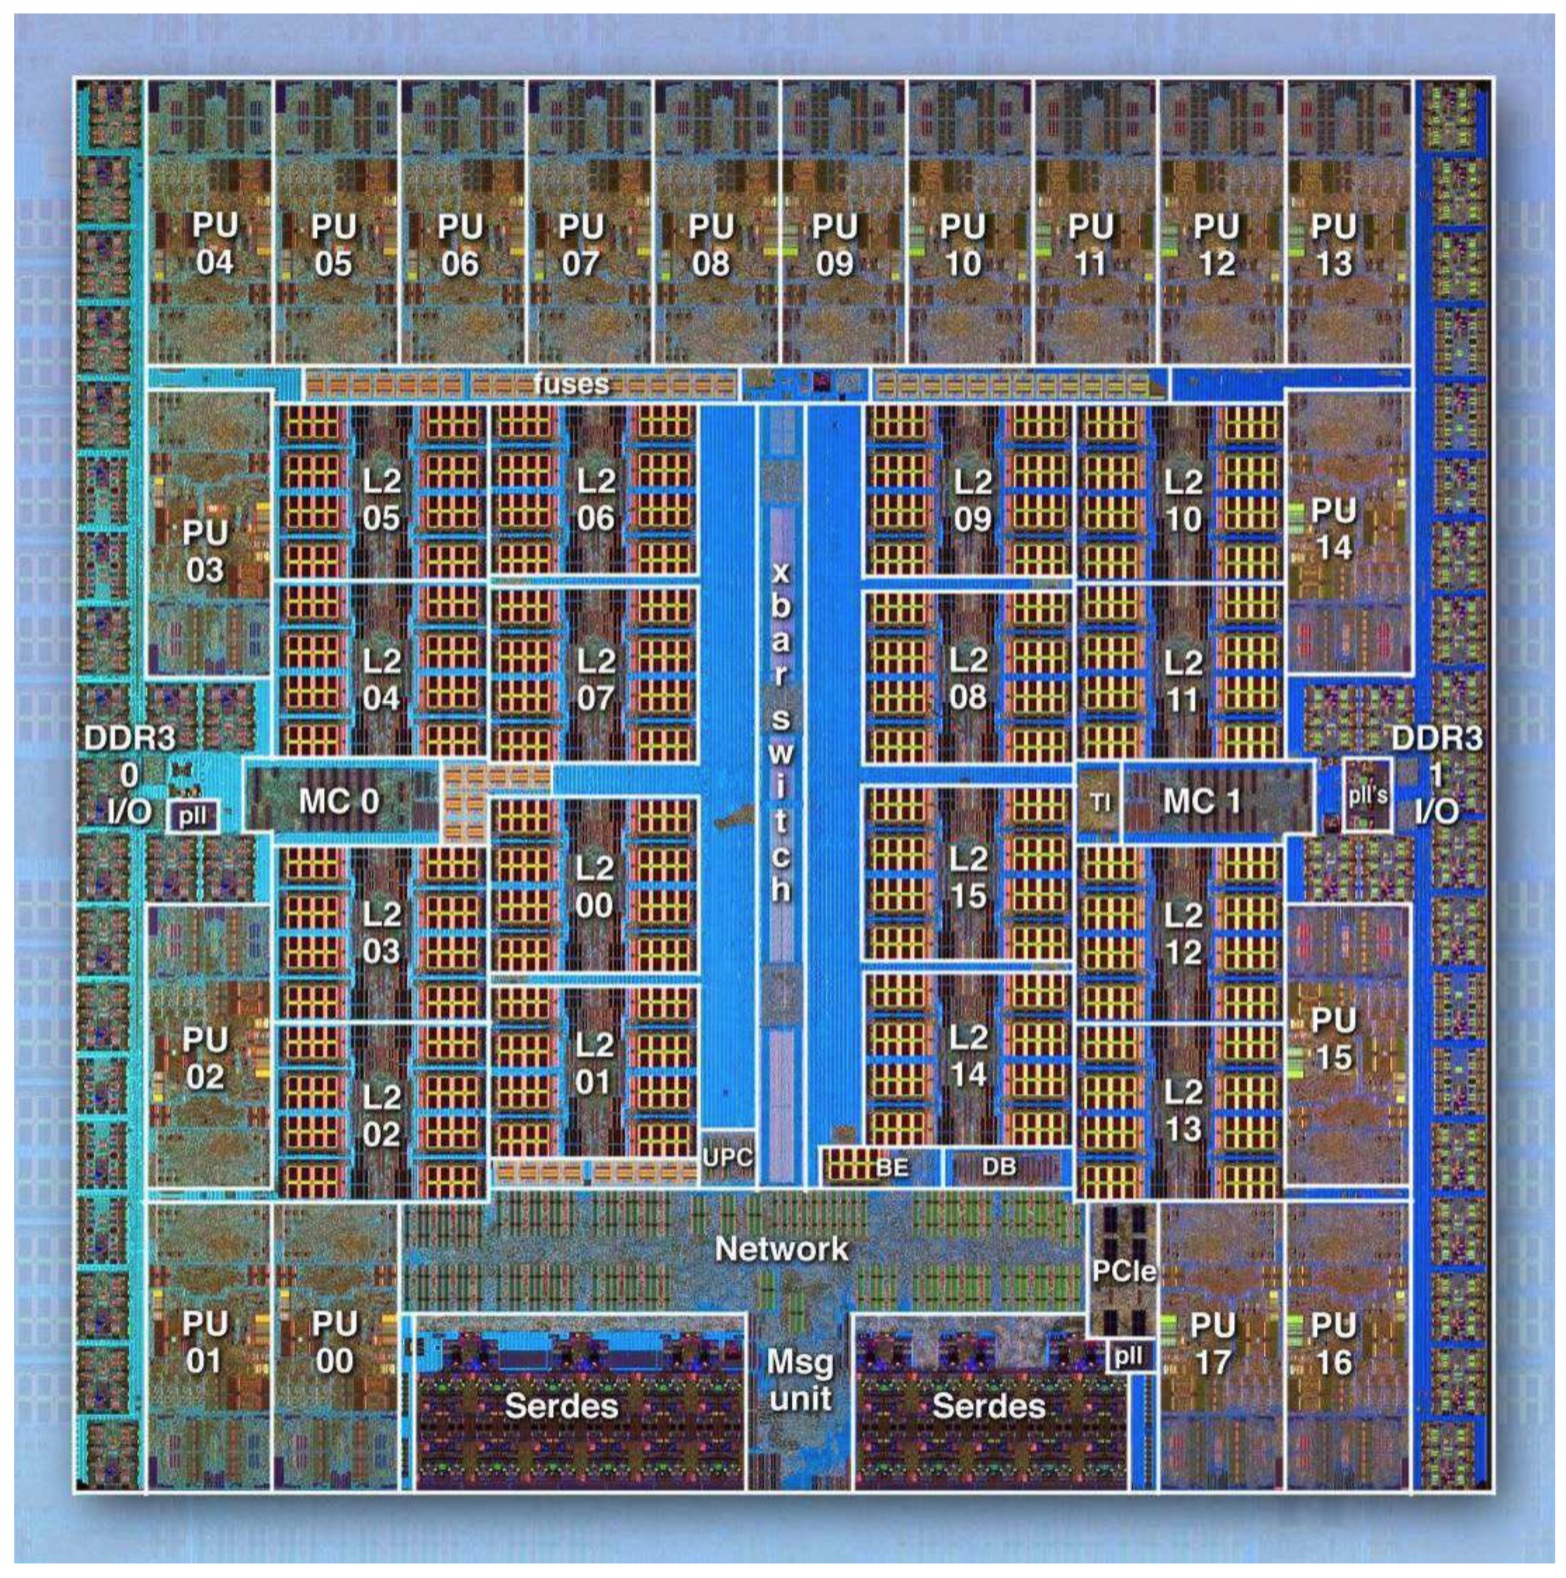
\includegraphics[width=\textwidth]{figures/A2processor.jpg}\\
      \small{IBM A2 System-on-a-Chip} \\
      \tiny{R.Haring, 2011, "The Blue Gene/Q Compute Chip"}
    \end{column}
  \end{columns}
\end{frame}

\begin{frame}
  \frametitle{Summit Computing Hardware}
  \textbf{Focus on GPUs; they provide 95\% of memory bandwidth and 98\% of FLOPs}
    \begin{columns}
    \begin{column}{0.7\textwidth}
  \begin{itemize}
    \item 6 V100 and 2 P9 per node
    \item 4,608 nodes $\rightarrow$ 27,648 V100 and 9,216 P9
  \end{itemize}
  {
  \begin{table}[]
    \begin{tabular}{lrr}
      Processor   & Double Precision & Memory           \\
                  & TeraFLOPs        & Bandwidth (GB/s) \\
      V100        & 7.5              & 900              \\
      P9          & 0.5              & 135       \\
      P9/V100     & 7\%              & 15\% \\
      \\
      Full System &                  & \\
      V100        & 207,360          & 24,833,200       \\
      P9          & 4,608            & 1,244,160       \\
      P9/V100     & 2\%              & 5\%
    \end{tabular}
  \end{table}
  }
  % Summit GPUs: 207PF, 24 PB/s
  % Summit P9s:  4.6PF, 1 PB/s
  %from sc18-tutorial-pleiter.pdf
    \end{column}
    \begin{column}{0.3\textwidth}
      \begin{figure}
        \centering
        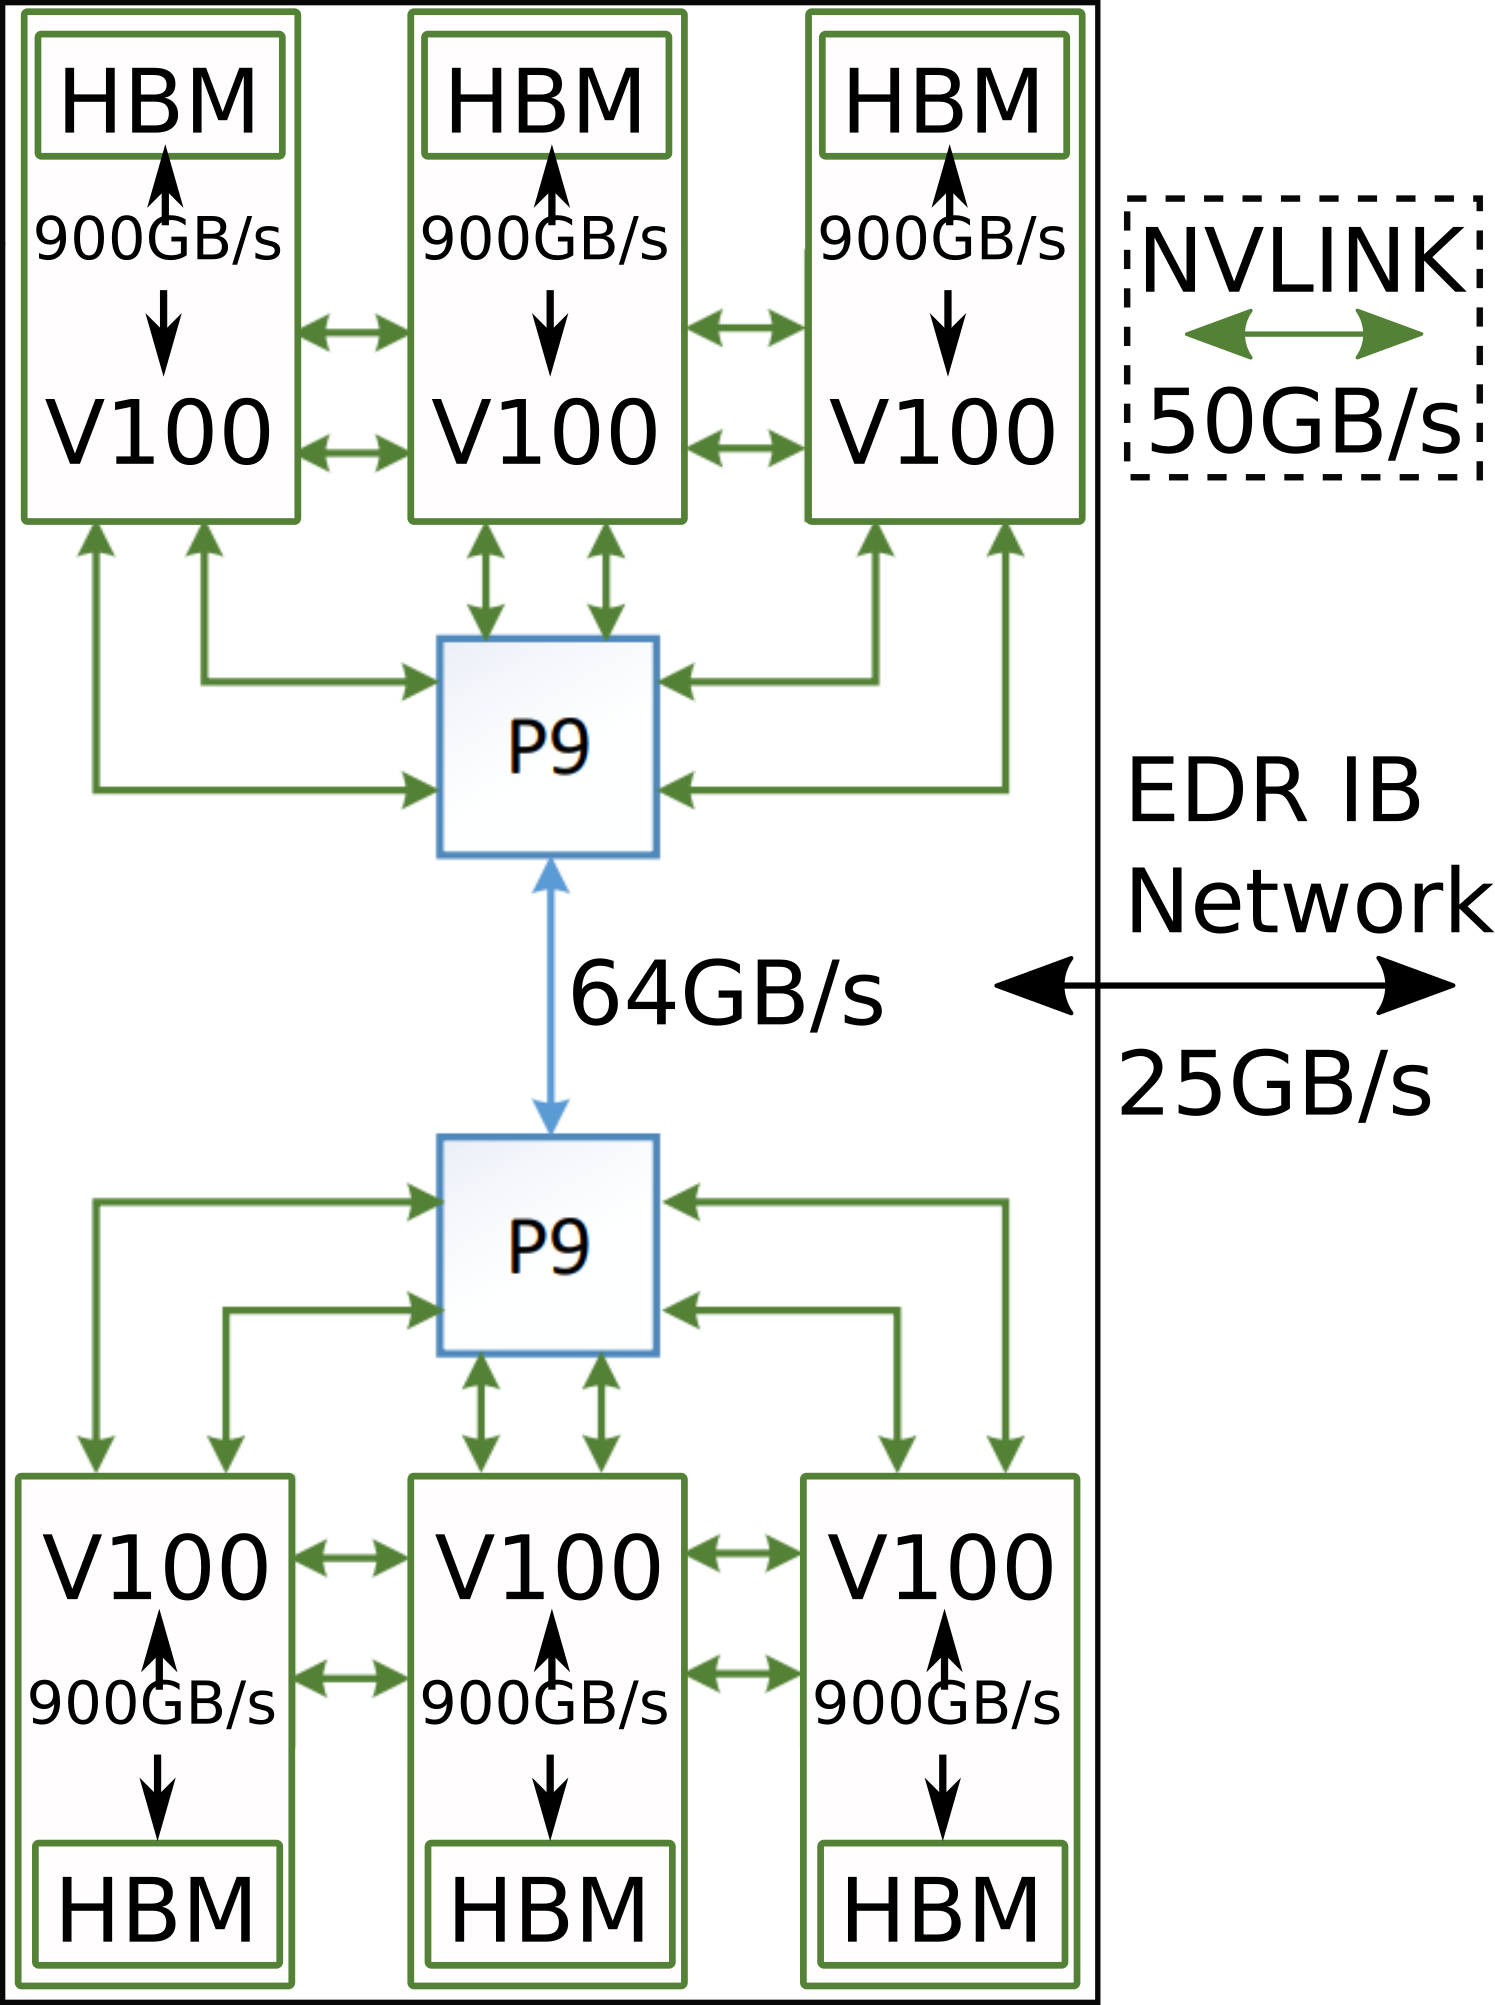
\includegraphics[width=.9\textwidth]{figures/summit-node.png}\\
        \tiny{J.Choquette. Hot Chips 2017. \\"Volta: Programmability and Performance"}
      \end{figure}
    \end{column}
    \end{columns}
\end{frame}

\begin{frame}
  \frametitle{Summit Communication Hardware}
  \textbf{Overlap communication with computation and minimize inter-node
  communication:\\
  205:1 ratio of aggregate V100 HBM bandwidth to inter-node EDR bandwidth}
    \begin{columns}
    \begin{column}{0.7\textwidth}
      \small
      \begin{table}[]
        \begin{tabular}{lrrr}
        System                      & Stream & Network & Stream/ \\
                                    & Triad  & Peak    & Network \\
                                    & (GB/s) & (GB/s)  & \\
        Summit (inter-node)         & 5,130  & 25      & 205     \\
        Summit (intra-node)         & 855    & 100     & 8.6     \\
        Stampede2                   & 194    & 12      & 17      \\
        Mira                        & 27     & 20      & 1.4 \\
        \hline
        Perlmutter (inter-node)[1] & 5,130  & 100     & 51   \\
        \hline
        \end{tabular}
      \end{table}
      {\small
        Summit stream/network ratios
        \begin{itemize}
          \item inter-node - sum six V100 HBM to EDR IB bandwidth
          \item intra-node - V100 HBM bandwidth to NVLINK bandwidth
        \end{itemize}
        [1] `4x Volta Next' ?= 4x1.5xV100, Slingshot 4x 25GB/s links
      }
    \end{column}
    \begin{column}{0.3\textwidth}
      \begin{figure}
        \centering
        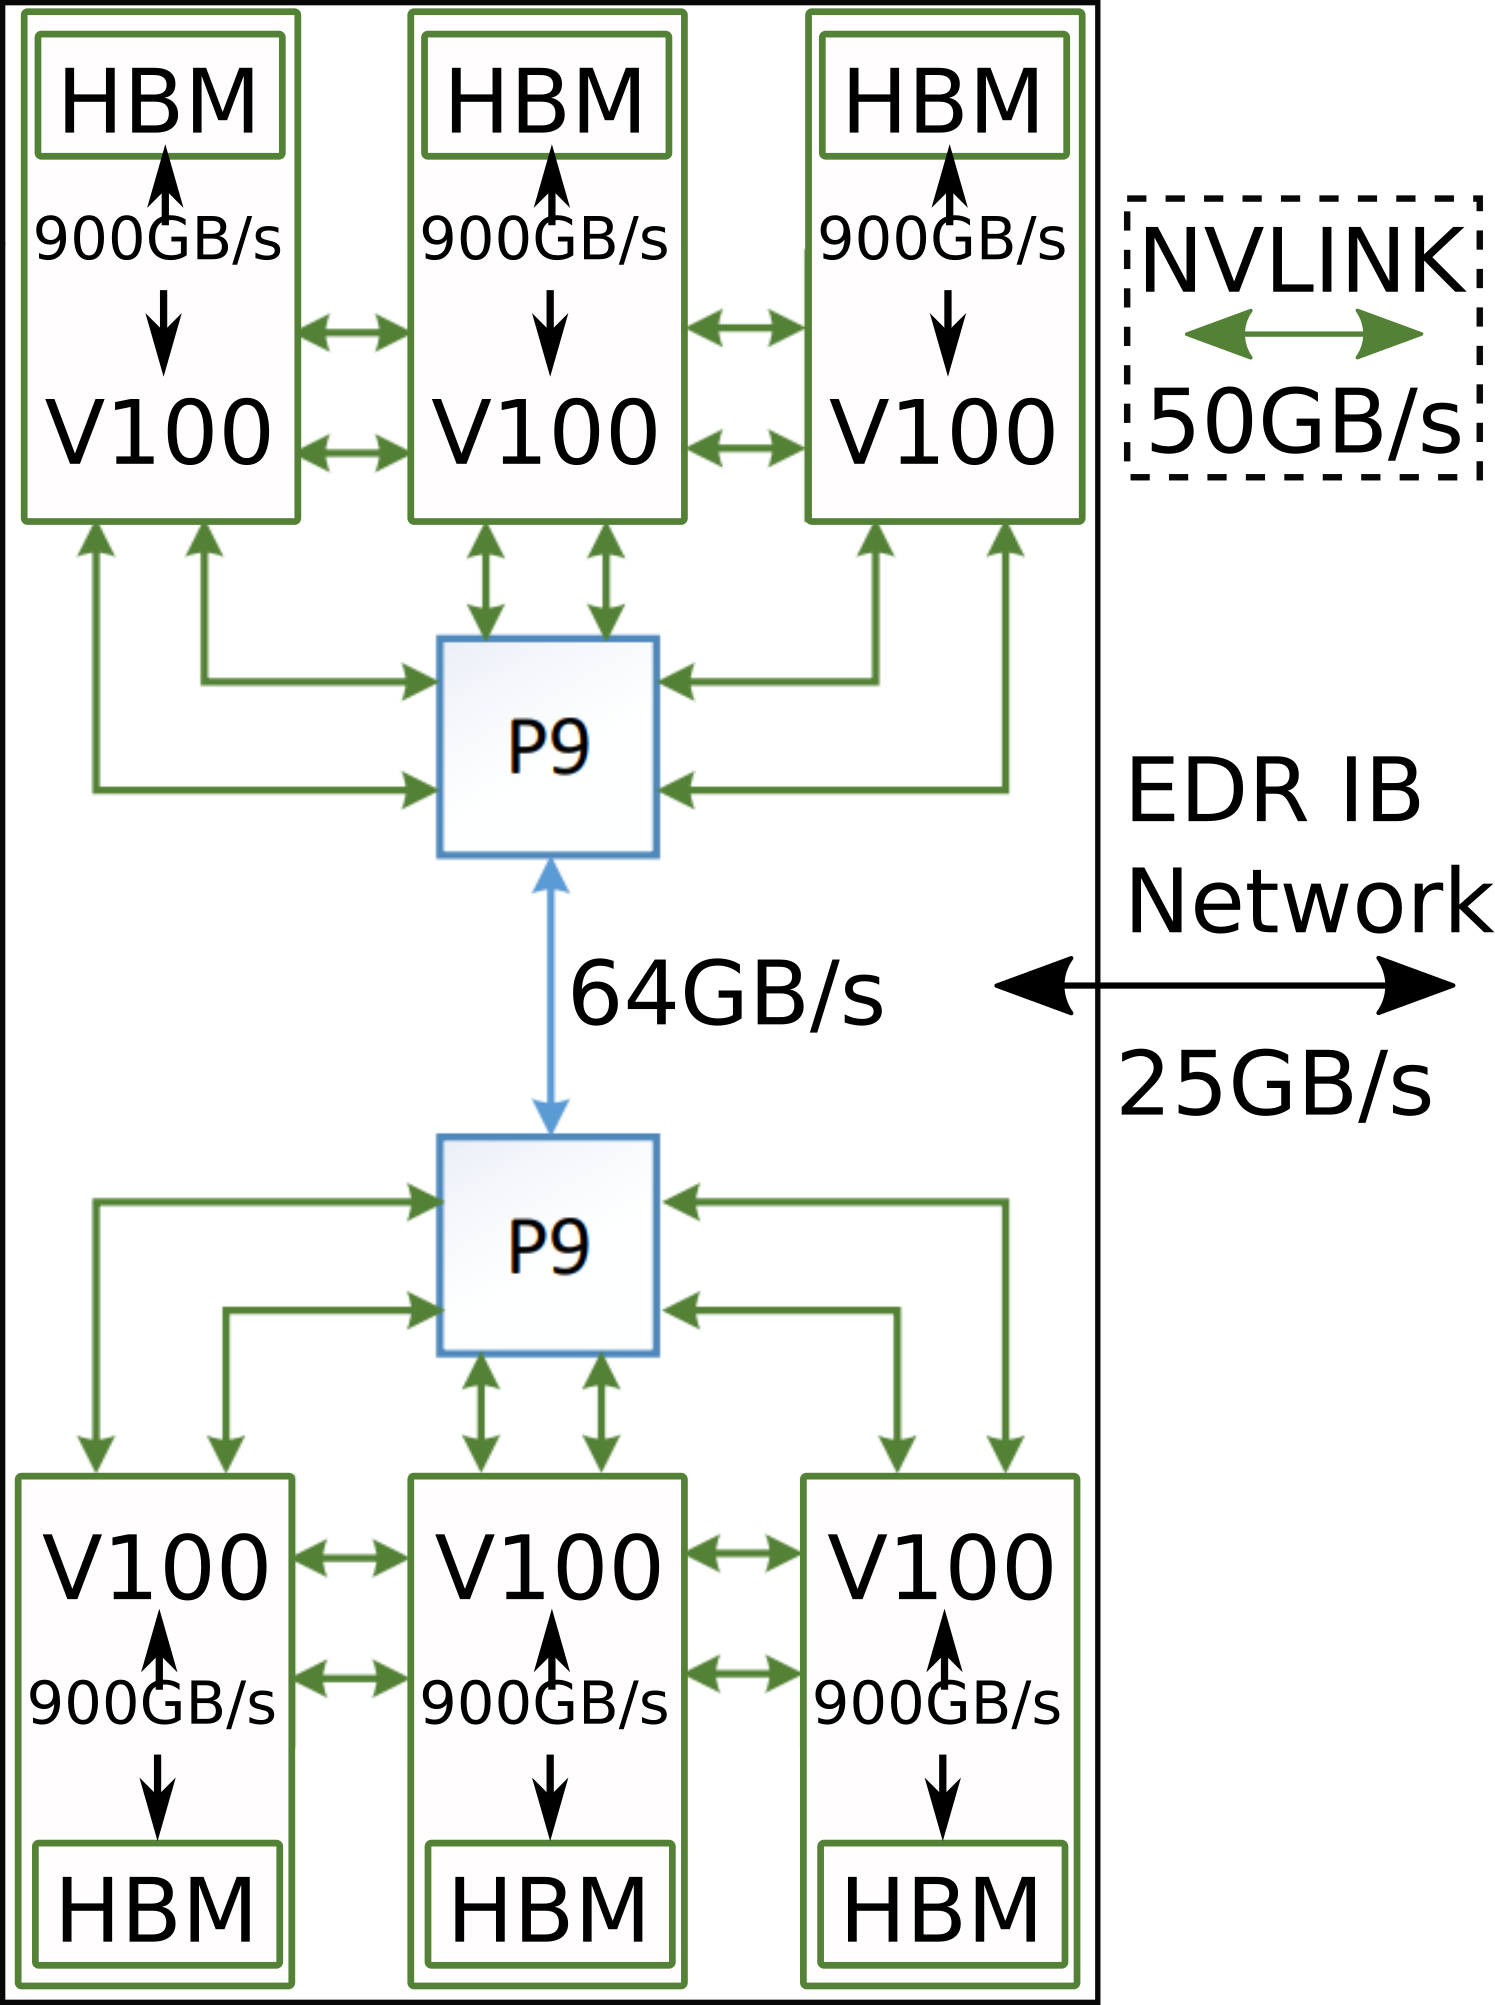
\includegraphics[width=.9\textwidth]{figures/summit-node.png}\\
        \tiny{J.Choquette. Hot Chips 2017. \\"Volta: Programmability and Performance"}
      \end{figure}
    \end{column}
  \end{columns}
  %V100 stream triad from Jack Choquette HotChips 2017 presentation "Volta: Programmability and Performance"
  %Mira network ref: PAMI: A Parallel Active Message Interface for the Blue Gene/Q Supercomputer
  %Mira stream triad ref: Bob Walkup "Application Performance Characterization and Analysis on Blue Gene/Q"
  %On a Skylake cluster like Stampede2 the ratio is in the range of 250:1 (~3 TFDP for two socket
  % skylake https://colfaxresearch.com/xeon-2017/ and
  % 12GB/s Omnipath https://portal.tacc.utexas.edu/user-guides/stampede2#overview-network)
  % SKX stream triad: "TACC Technical Report TR-17-01 Benchmarking the Intel Xeon Platinum 8160 Processor"
\end{frame}

%----------------------------------------------------------------------%
%----------- Section --------------------------------------------------%
%----------------------------------------------------------------------%
\section{Partitioning and Load Balancing}
\begin{frame}
  \frametitle{Motivation and Focus}
  \begin{columns}
    \begin{column}{0.7\textwidth}
      Simulations with regions of physical interest that change.\\
      \smallskip
      Many simulations have one or more of the following
      characteristics that make scaling and achieving
      performance difficult.
      \begin{itemize}
        \item Complex relational structures.
        \item Irregular forms of computational and communication costs.
        \item Evolving imbalance of work characterized by multiple criteria.
      \end{itemize}

      Evolving simulations we focus on have:
      \begin{itemize}
        \item A single executable built from library APIs - in-memory
          interactions
        \item Bulk synchronous parallel execution model\\
          {\small \texttt (1) work (2) communicate (3) goto 1}
      \end{itemize}
    \end{column}
    \begin{column}{0.3\textwidth}
      \begin{figure}
        \centering
        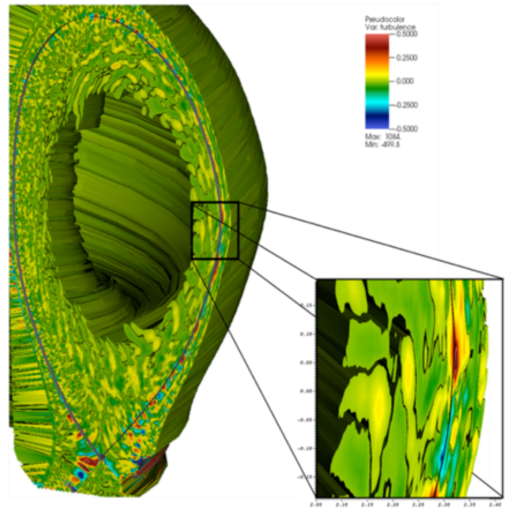
\includegraphics[width=.75\textwidth]{figures/xgcCase.png} \\
        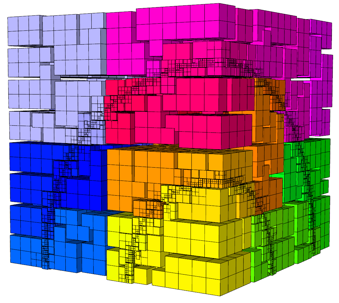
\includegraphics[width=.75\textwidth]{figures/laghos_sedov.png}\\
        \tiny{XGC fusion plasma physics (top) and MFEM Laghos Sedov blast
        (bottom)}
      \end{figure}
    \end{column}
  \end{columns}
\end{frame}

\begin{frame}
  \frametitle{Common Methods for Partitioning and Load Balancing}
  \begin{columns}
    \begin{column}{0.4\textwidth}
      \begin{itemize}
        \item Multilevel Graph Methods %Discuss poor scaling
          \begin{itemize}
            \item ParMETIS
            \item Zoltan
          \end{itemize}
        \item Geometric Methods %Require coordinates
          \begin{itemize}
            \item Recursive Coordinate(Inertial) Bisection
            \item Multi-Jagged
          \end{itemize}
        \item Diffusive Methods %Improve a partition efficiently
          \begin{itemize}
            \item Label Propagation
            \item ParMA and EnGPar
          \end{itemize}
        \item ... Not within a SIMT GPU
          \begin{itemize}
            \item same work for each thread
            \item e.g.) loop collapsing graph traversal - operate on edges
              instead of nodes
          \end{itemize}
      \end{itemize}
    \end{column}
    \begin{column}{0.6\textwidth}
      \begin{figure}
        \centering
        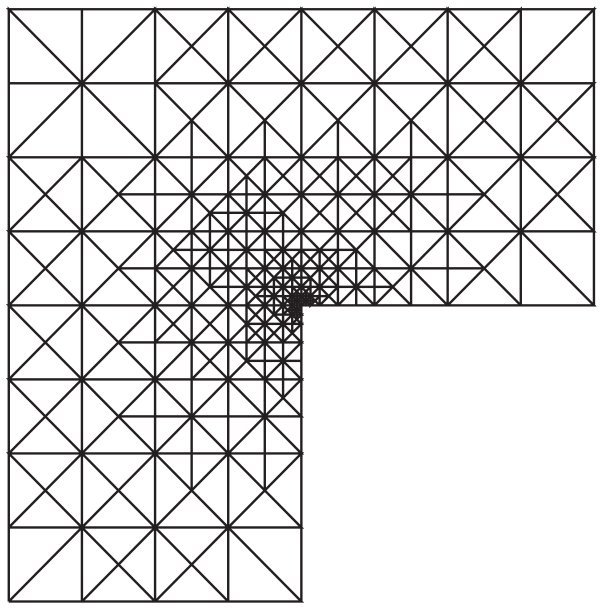
\includegraphics[width=.32\textwidth]{figures/mitchellMesh.png}
        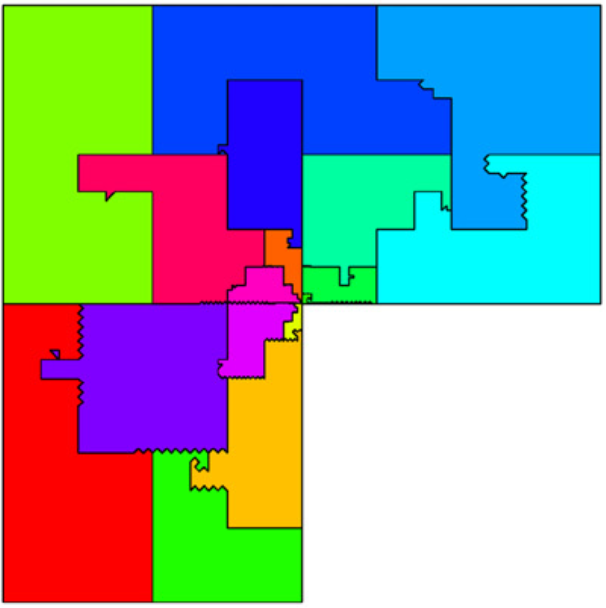
\includegraphics[width=.32\textwidth]{figures/mitchellHSFC.png}
        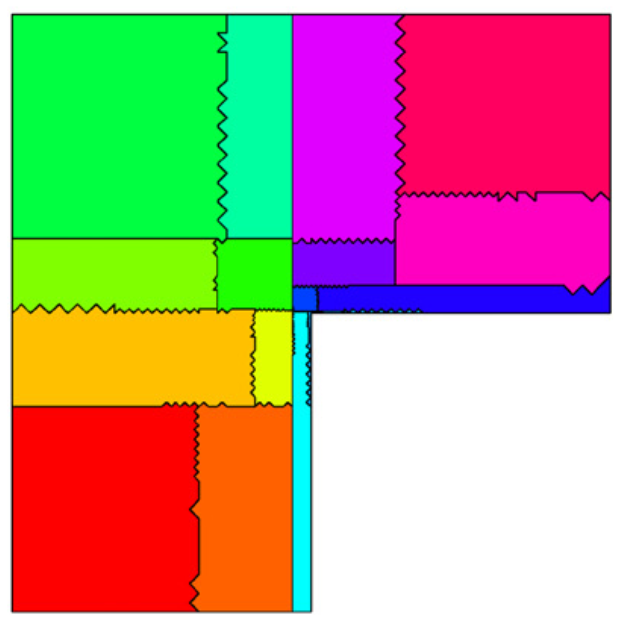
\includegraphics[width=.32\textwidth]{figures/mitchellRCB.png} \\
        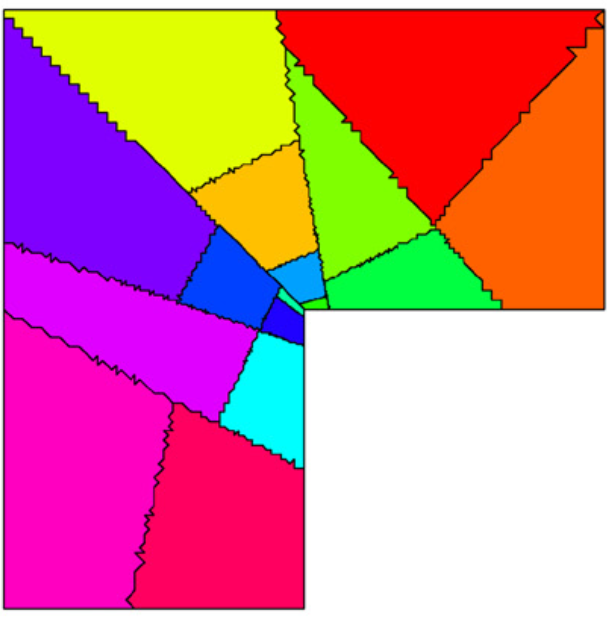
\includegraphics[width=.32\textwidth]{figures/mitchellRIB.png}
        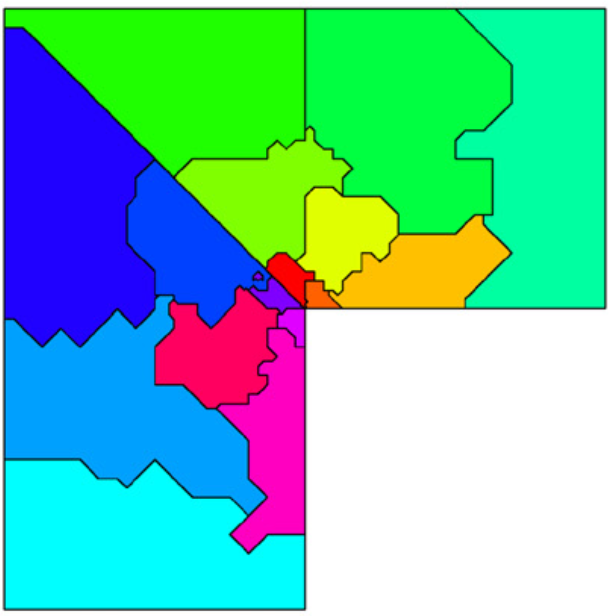
\includegraphics[width=.32\textwidth]{figures/mitchellParmetis.png} \\
        \small{Top to bottom, left to right: mesh, space filling curve,
        coordinate bisection, inertial bisection, multi-level k-way.} \\
        \tiny{``A refinement-tree based partitioning method for dynamic load
        balancing with adaptively refined grids'', William F. Mitchell}
      \end{figure}
    \end{column}
  \end{columns}
\end{frame}

\section{EnGPar - a graph based diffusive load balancer}
\begin{frame}
  \frametitle{}
  \center \huge{EnGPar: One Approach to Partition Control}
\end{frame}

\begin{frame}
  \frametitle{What is EnGPar?}
      \begin{itemize}
        \item Provides a diffusive load balancing algorithm for partition improvement and supports multi-criteria partitioning.
        \item Complements existing multi-level and geometric methods.
        \item Utilizes a weighted multi(hyper)graph structure to represent
          data dependencies.
        \item Implemented to support efficient data parallel operations on accelerators
      \end{itemize}
      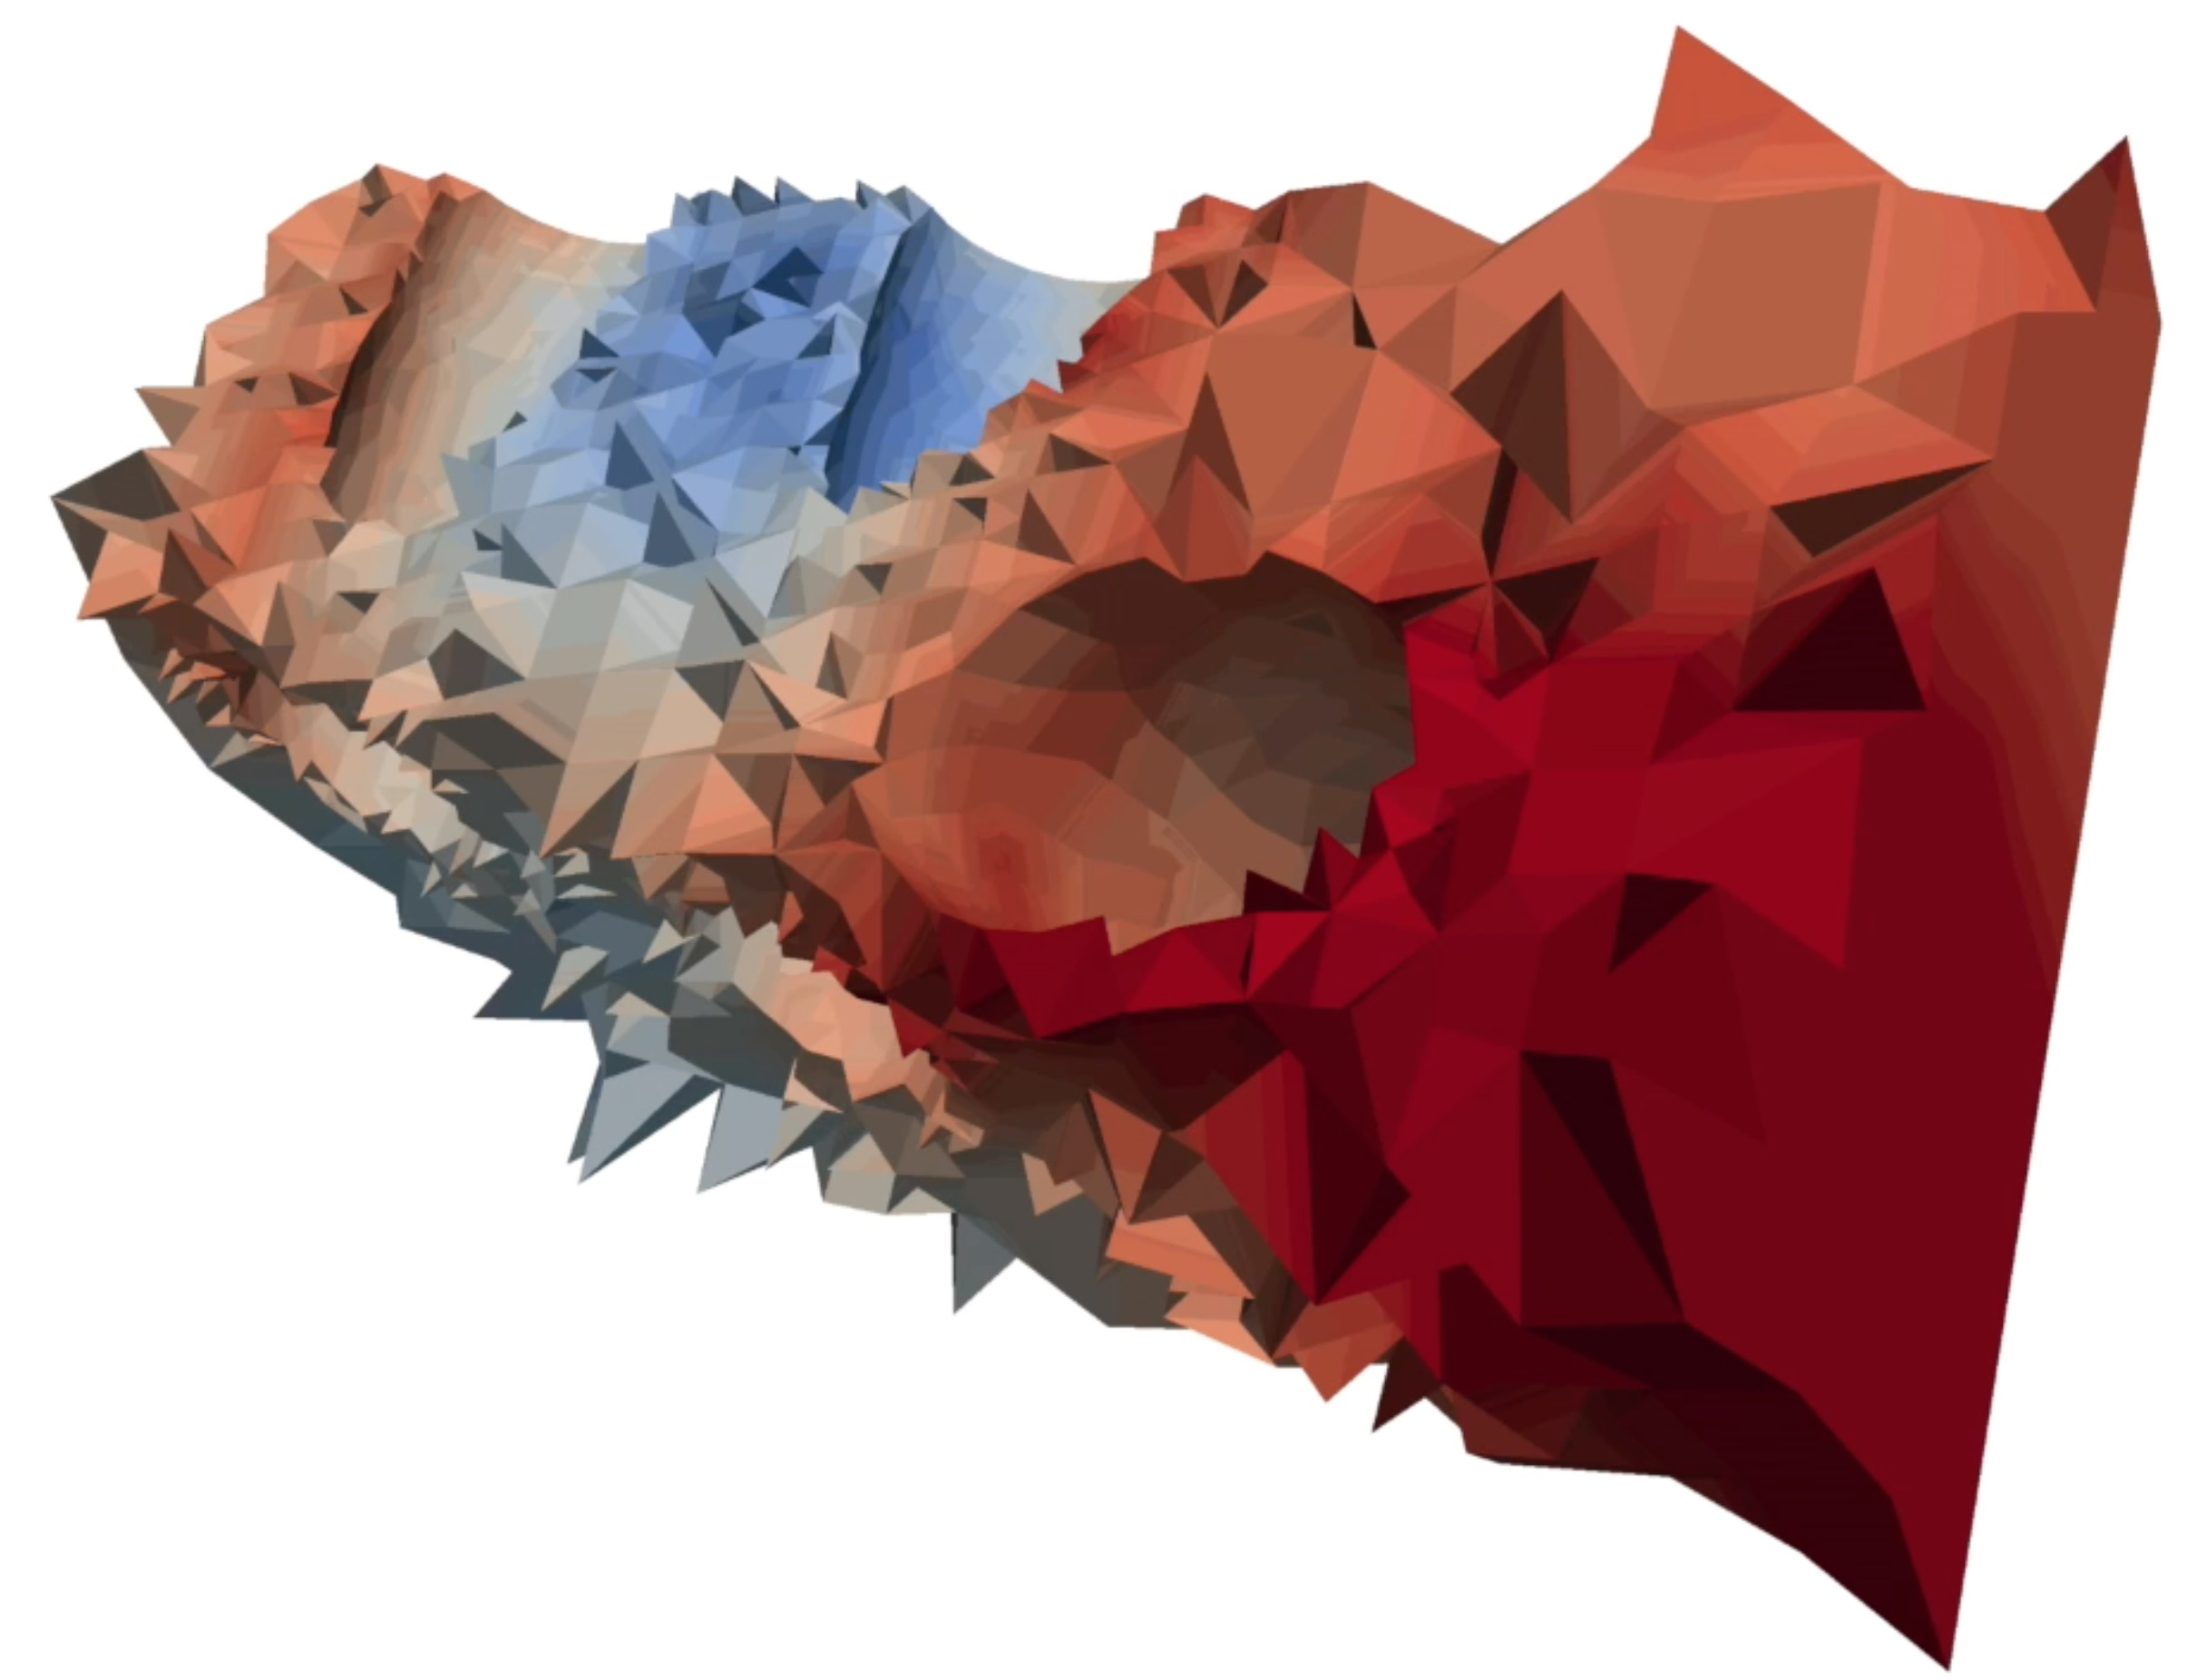
\includegraphics[width=.2\textwidth]{figures/engparDiffusion/0.jpg}
      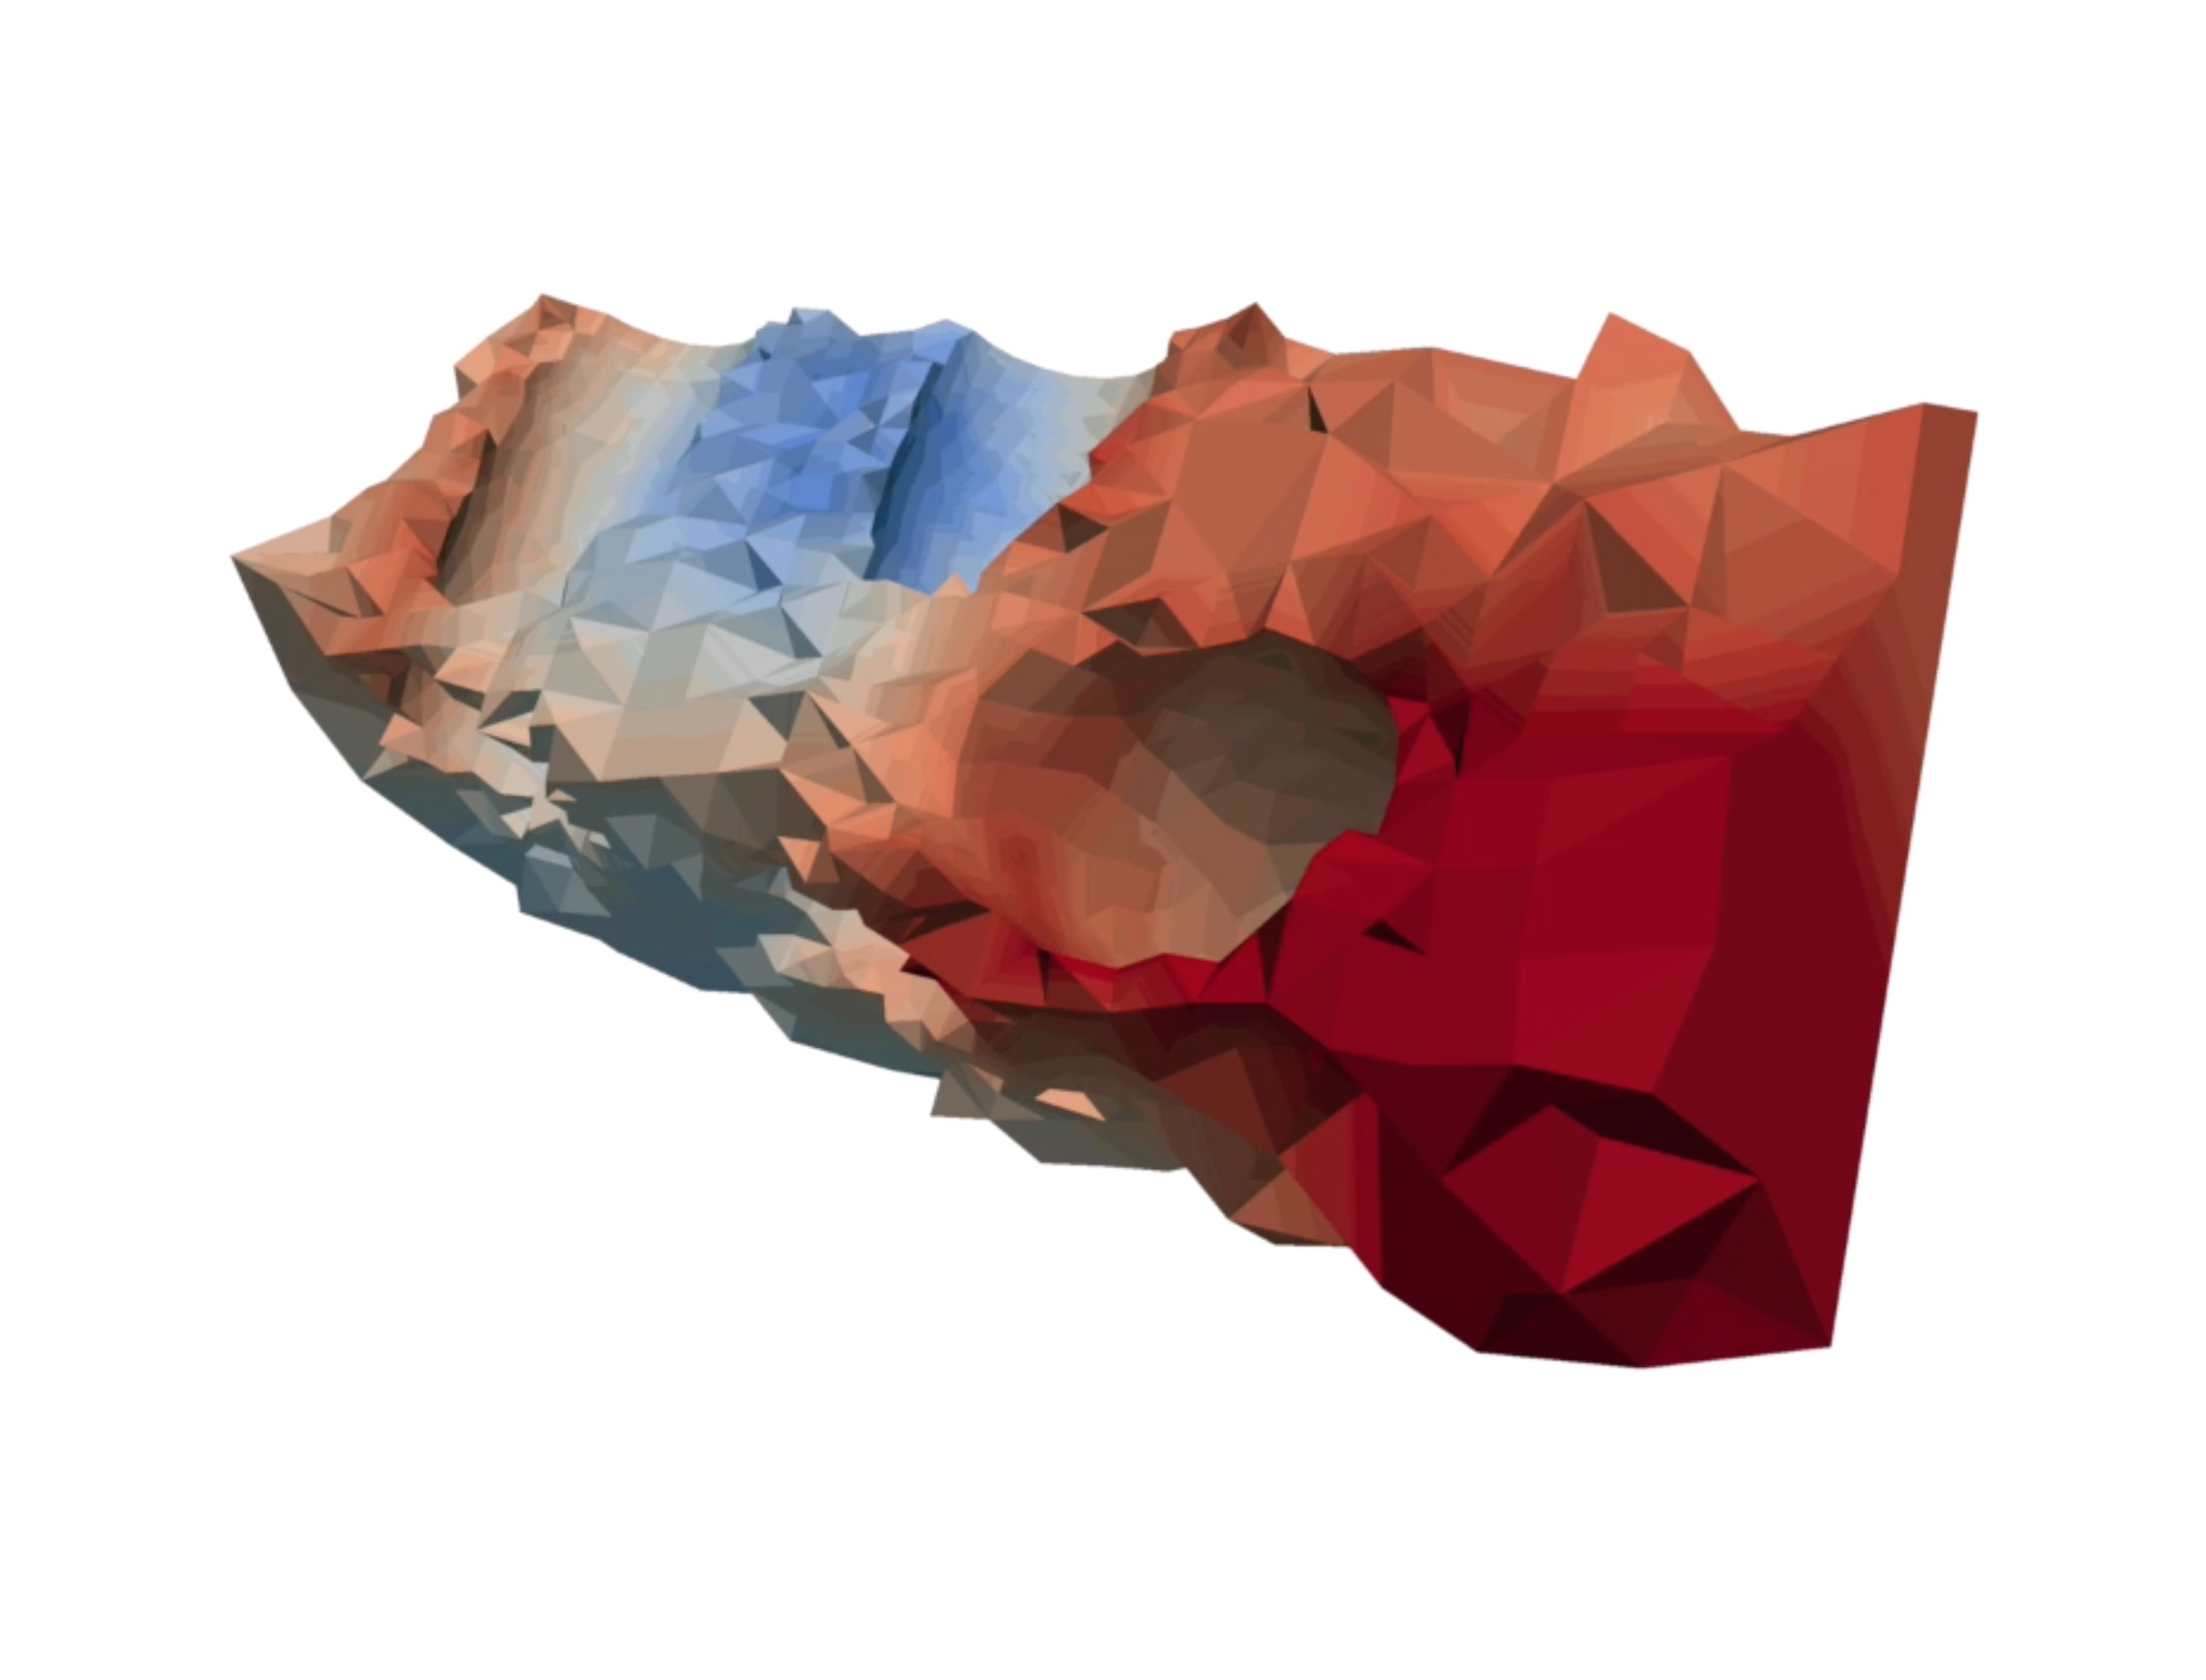
\includegraphics[width=.2\textwidth]{figures/engparDiffusion/1.jpg}
      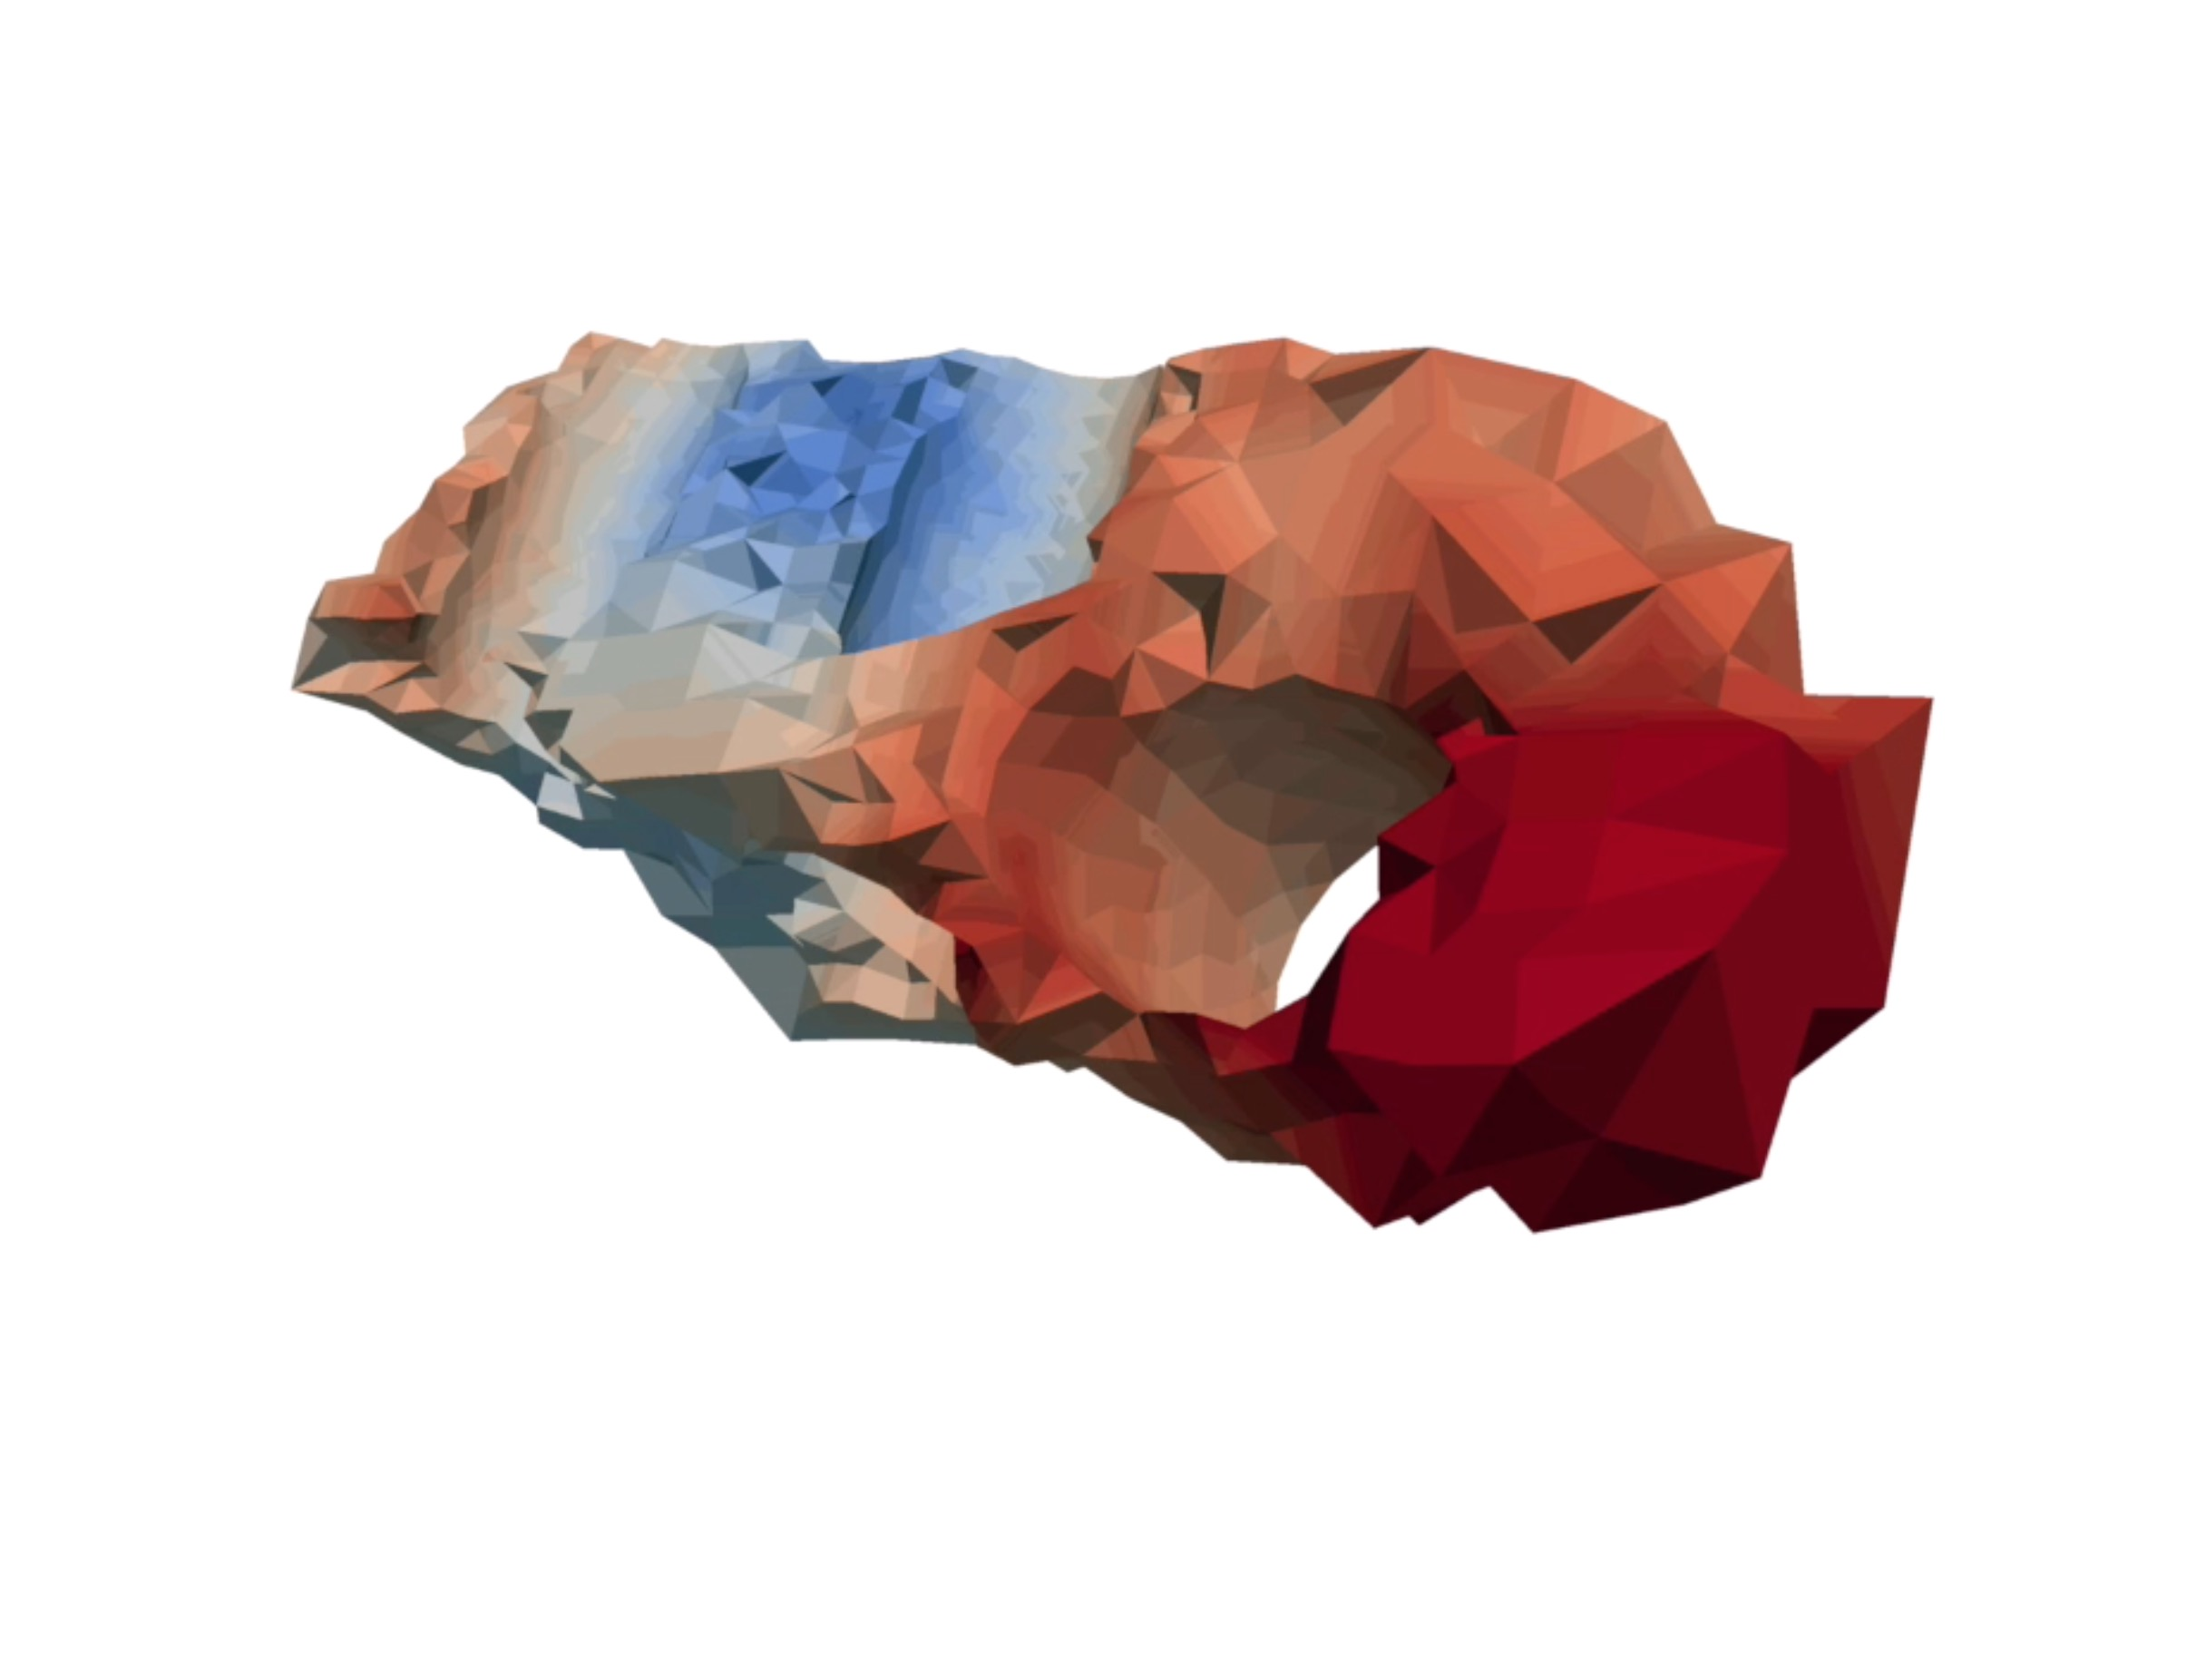
\includegraphics[width=.2\textwidth]{figures/engparDiffusion/2.jpg}
      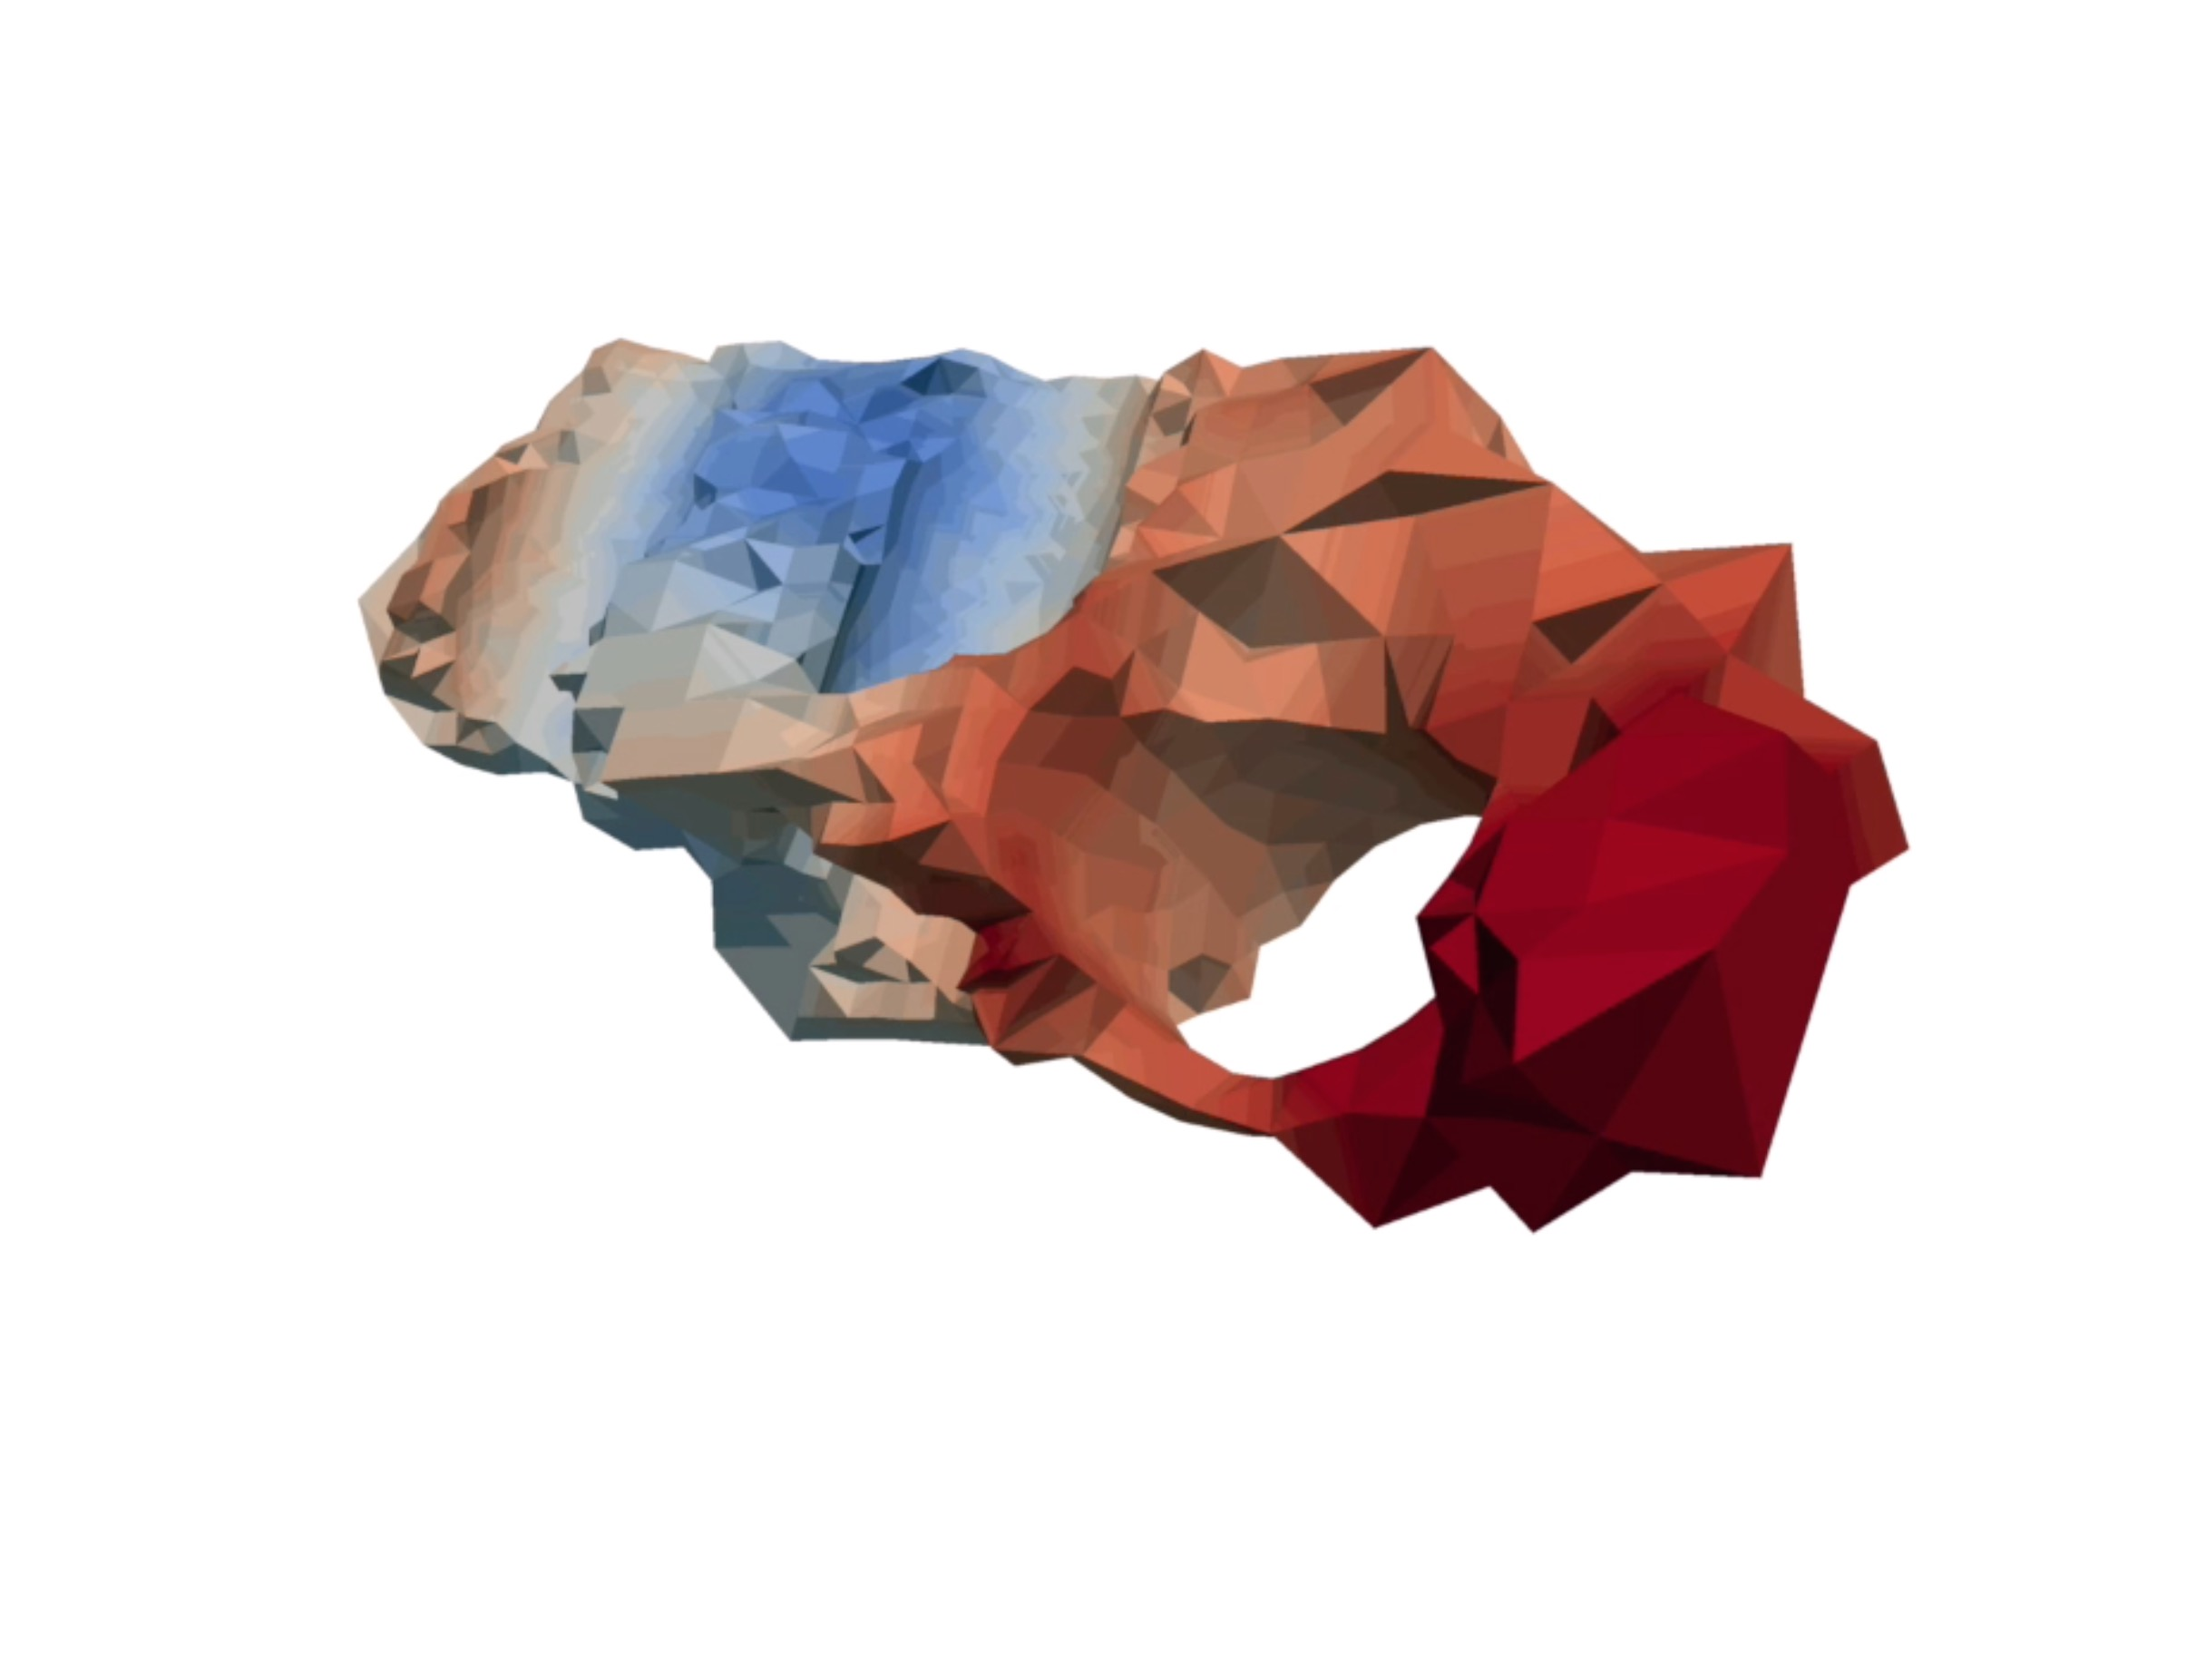
\includegraphics[width=.2\textwidth]{figures/engparDiffusion/3.jpg}
      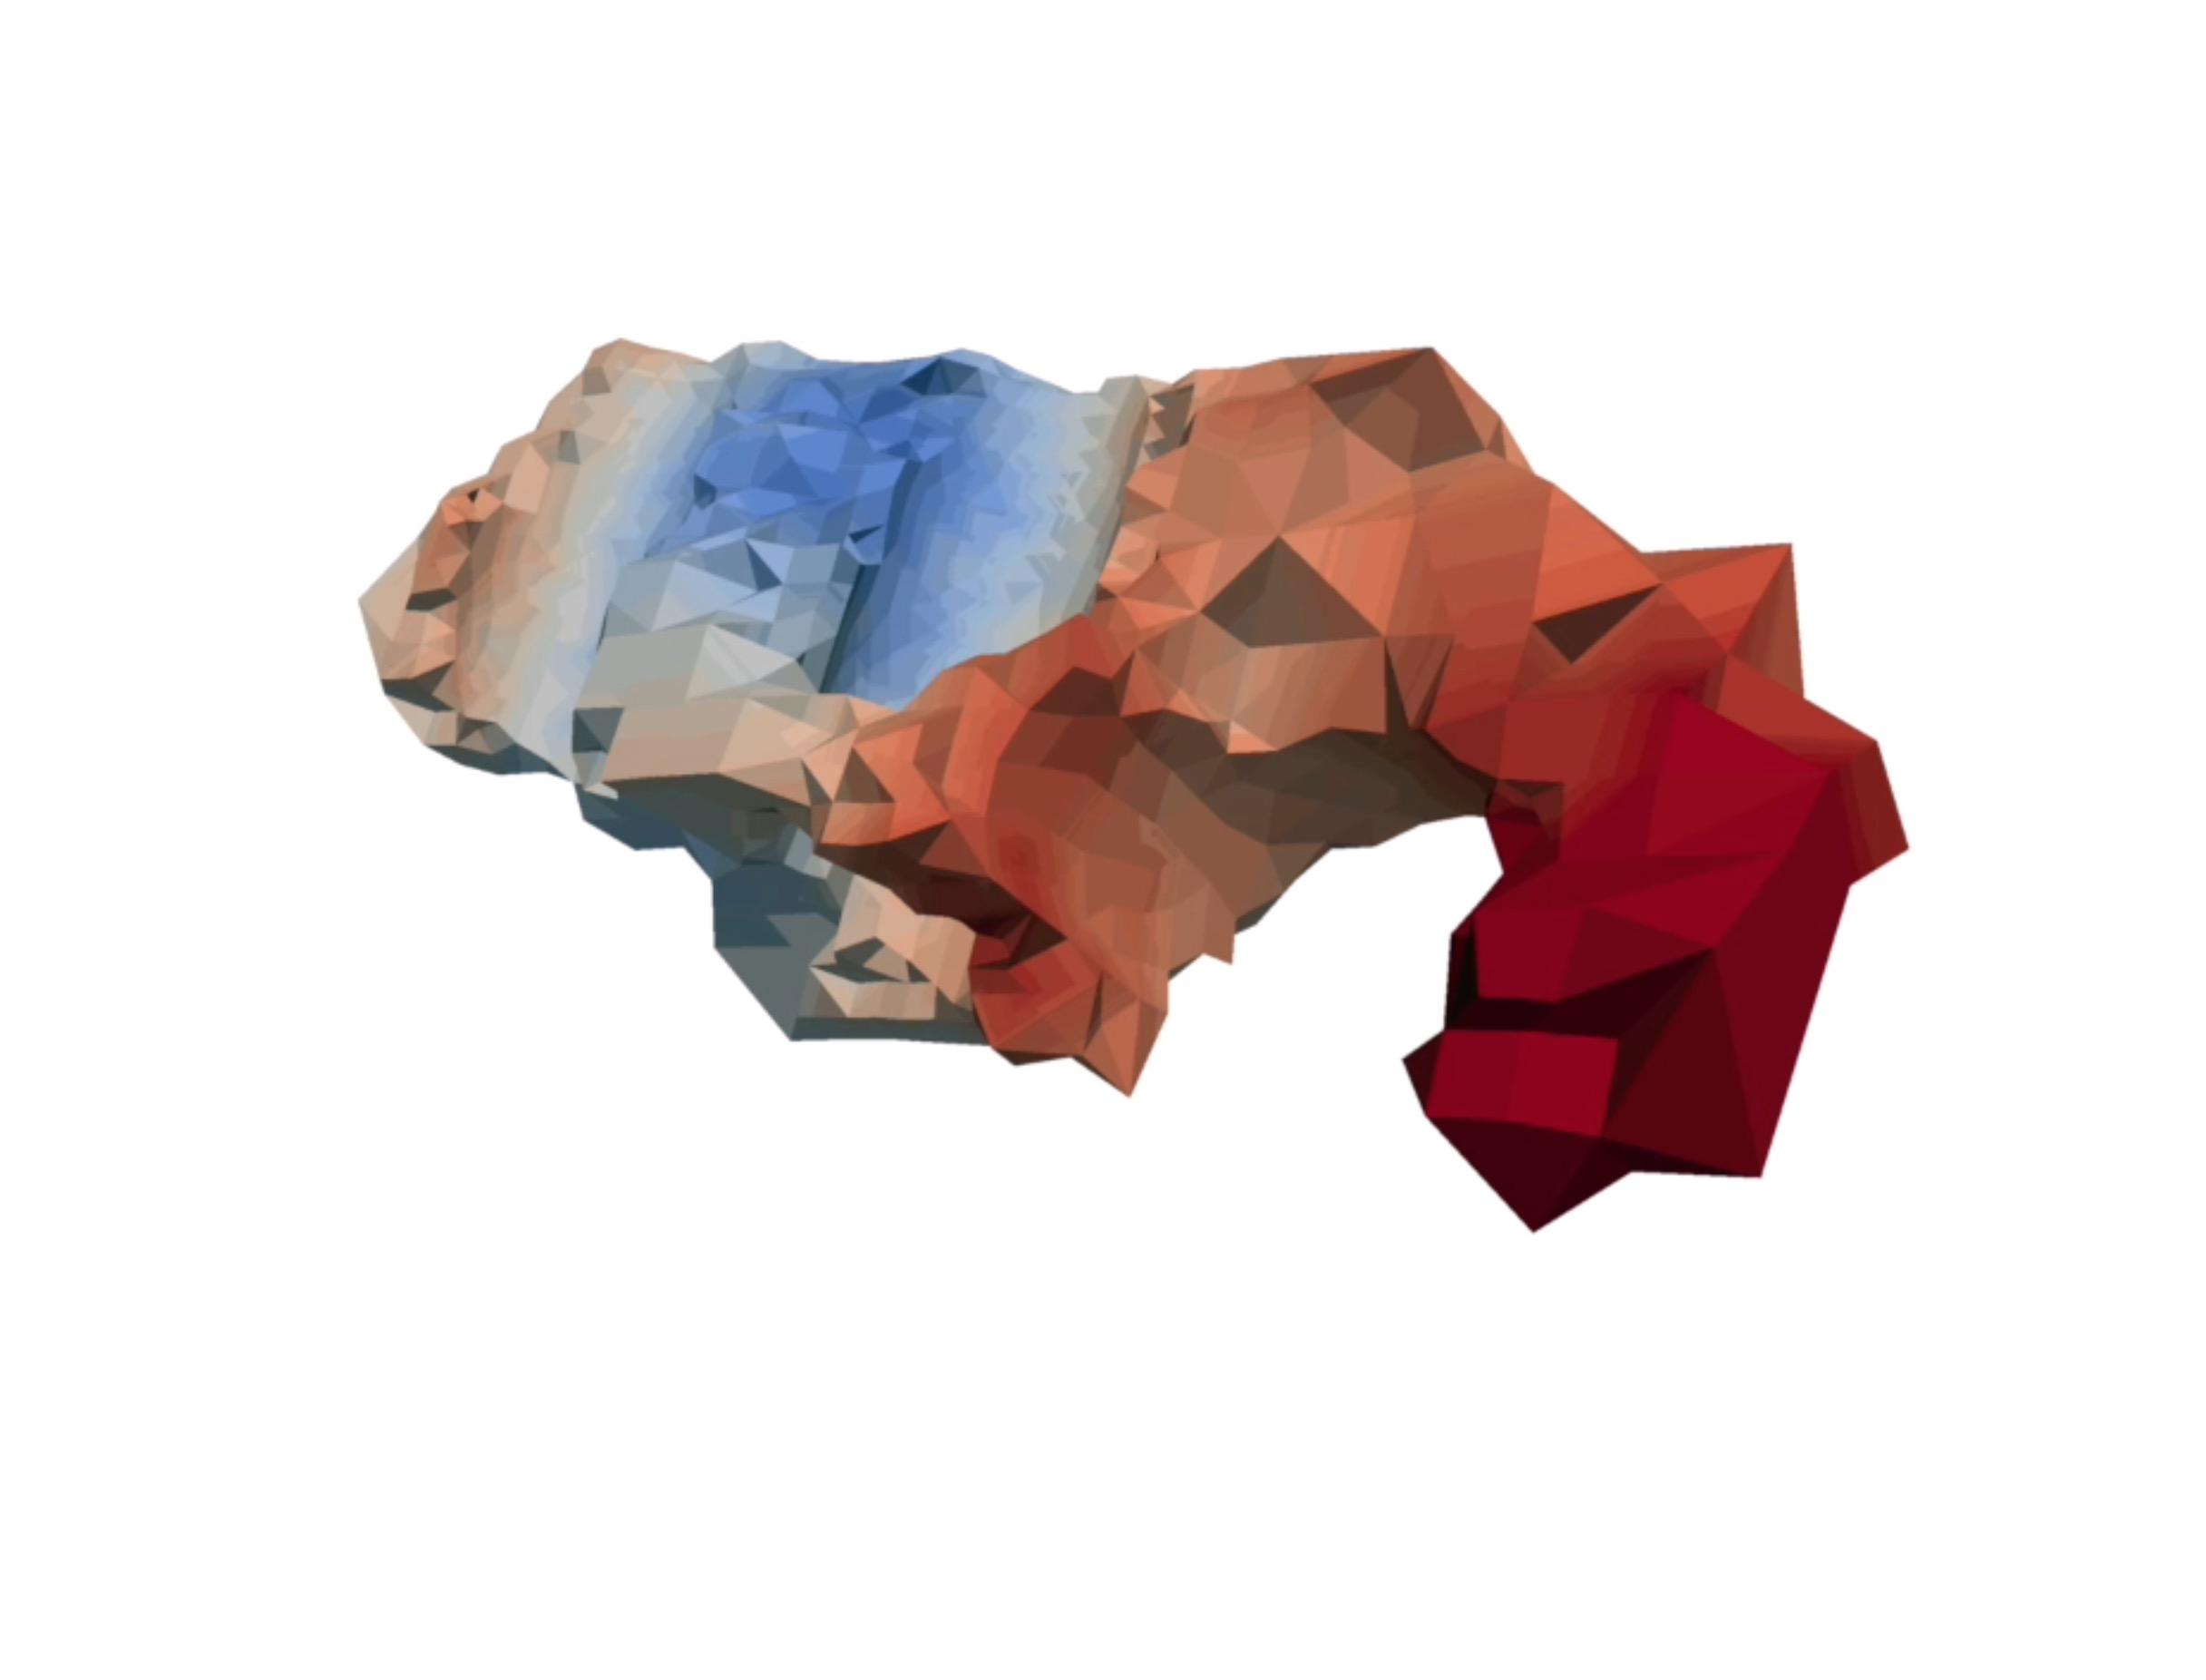
\includegraphics[width=.2\textwidth]{figures/engparDiffusion/4.jpg}
      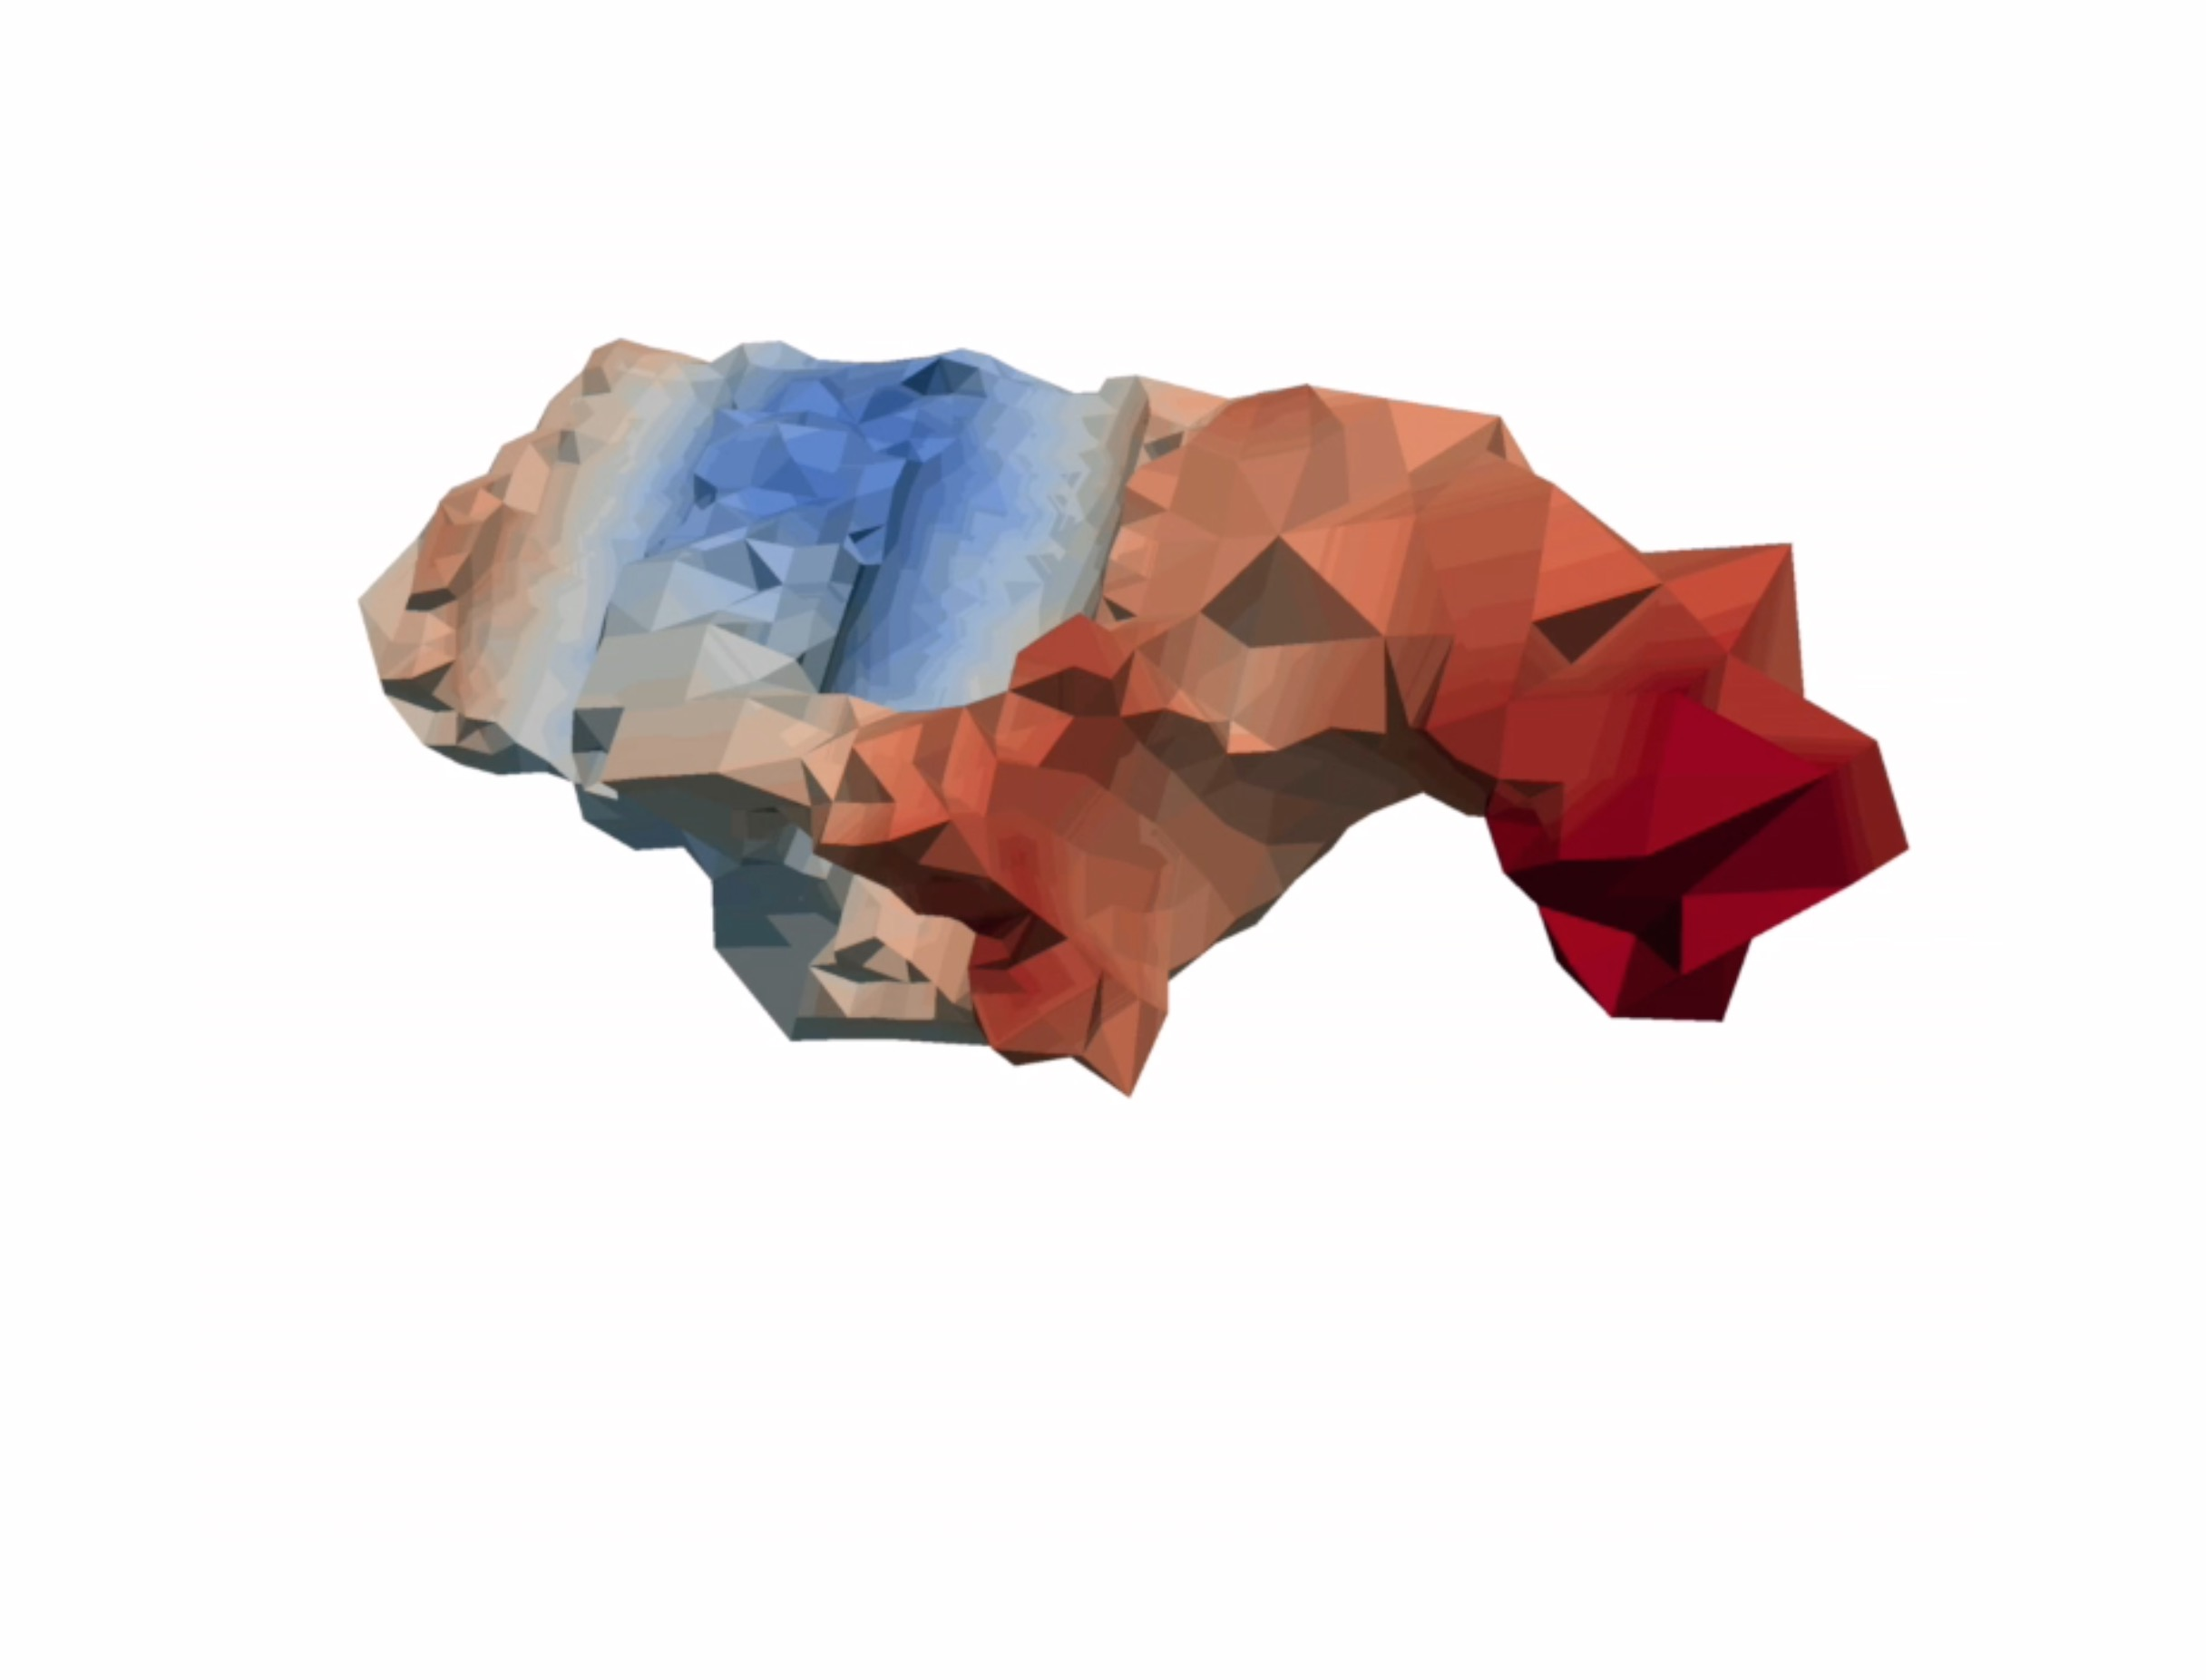
\includegraphics[width=.2\textwidth]{figures/engparDiffusion/5.jpg} \\
      \small{Multiple diffusive iterations (left to right) biased
      to migrate entities in order of descending distance (red to blue) from the
      topological center of the part (blue).}
\end{frame}

\begin{frame}
  \frametitle{Unstructured Mesh Partition Improvement}
  \medskip
  Problem setup
  \begin{itemize}
    \item Billion element mesh of vertical tail structure.
    \item Run on the Mira BG/Q with one process per hardware thread.
    \item Target imbalance of 1.05.
    \item The imbalance of a given type (vtx, edge,
      face, or region) is defined as the max part
      weight divided by the avg part weight.
  \end{itemize}
  Initial partitions are built using:
  \begin{itemize}
  \item Global ParMETIS part k-way to 8Ki($8*2^{10}$) parts.
  \item Local ParMETIS part k-way from 8Ki to 128Ki, 256Ki, and 512Ki parts.
  \end{itemize}
  The partitions before using EnGPar:\\
  \begin{table}[!h]
    \small
    \centering
    \begin{tabular}{||c|c|c|c||}
      \hline
      Number of Parts &128Ki&256Ki&512Ki \\
      \hline
      Elements per part & 9,836 & 4,918&2,459  \\
      \hline
      Vertex imbalance & 1.13 & 1.18 & 1.53 \\
      \hline
      Element imbalance & 1.02& 1.02& 1.02\\
      \hline
    \end{tabular}
  \end{table}
\end{frame}

\begin{frame}
  \frametitle{Element Partition: Mesh Vertex and Element Imbalance}
  \begin{figure}
    \centering
    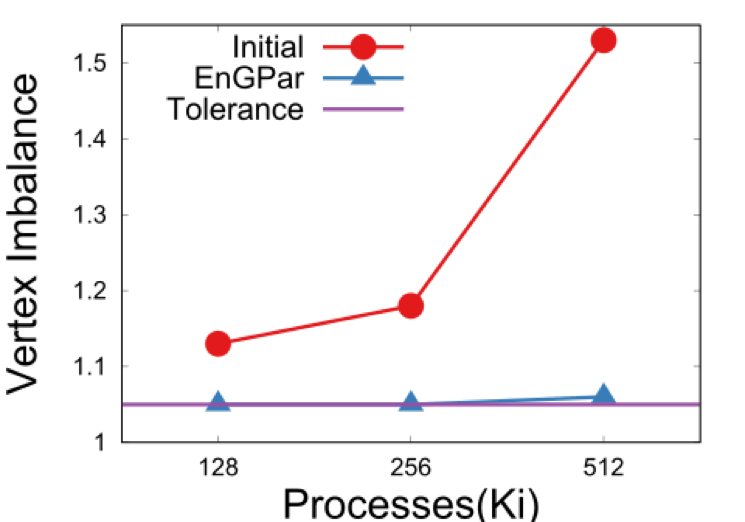
\includegraphics[width=.49\textwidth]{../accelerated_cse19/figures/elmPtn_vtxImb.png}
    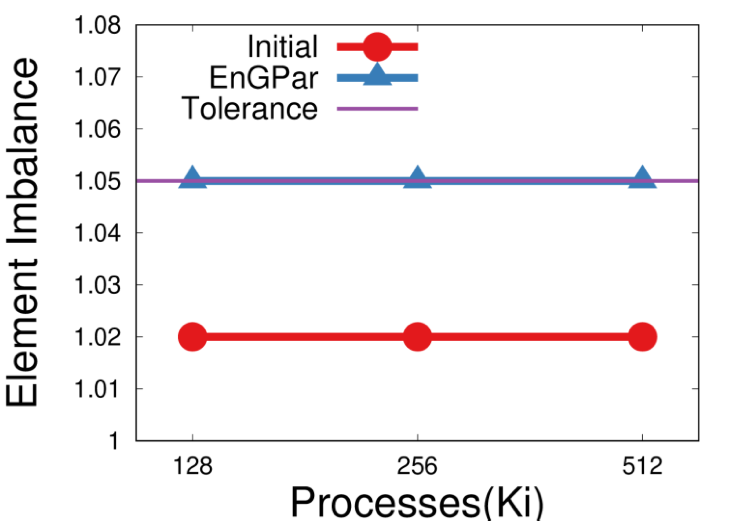
\includegraphics[width=.49\textwidth]{../accelerated_cse19/figures/elmPtn_elmImb.png} \\
    Mesh vertex imbalances is reduced from 13\% to 5\% for 128Ki, 18\% to 5\% for
    256Ki, and 53\% to 6\% for 512Ki.  Edge cut is increased by 1\%.
  \end{figure}
\end{frame}


\section{Load Balancing On Accelerated Systems}

\begin{frame}
  \frametitle{}
  \center \huge{Balancing High-order Adaptive Finite Elements}
\end{frame}

\begin{frame}
  \frametitle{MFEM Laghos MiniApp - High-order Compressible Gas Dynamics}
  Tzanio Kolev and Vladimir Tomov, Lawrence Livermore National Laboratory \\
  DOE Exascale Computing Project: The Center for Efficient Exascale Discretizations (CEED)
  \begin{columns}
    \begin{column}{0.5\textwidth}
      Goals
      \begin{itemize}
	\item Help applications leverage future architectures by providing them high
          order unstructured mesh methods.
        \item Collaborate with hardware vendors and software projects to guide
          the design of upcoming exascale systems.
      \end{itemize}
    \end{column}
    \begin{column}{0.5\textwidth}
      \begin{figure}
        \centering
        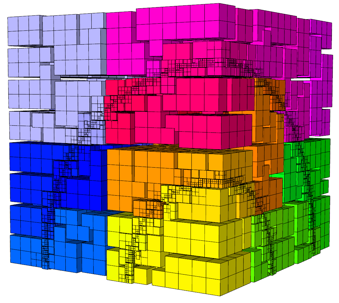
\includegraphics[width=.7\textwidth]{figures/laghos_sedov.png} \\
        \tiny{The Laghos miniapp's Sedov blast wave problem.  Laghos solves the
        time-dependent Euler equation of compressible gas dynamics in a moving
        Lagrangian frame using high-order finite element spatial discretization
        and explicit high-order time-stepping.}
      \end{figure}
    \end{column}
  \end{columns}
\end{frame}

\begin{frame}
  \frametitle{MFEM Laghos MiniApp - Partitioning Approach (T. Kolev, V. Tomov)}
  \begin{columns}
    \begin{column}{0.5\textwidth}
      \begin{itemize}
	\item One MPI process per GPU
        \item Initial partition with METIS
        \item Non-conforming adaptive mesh refinement (AMR) version using space
          filling curves
        \item GPU porting of computationally dominant functions in AMR version is underway
      \end{itemize}
    \end{column}
    \begin{column}{0.5\textwidth}
      \centering
      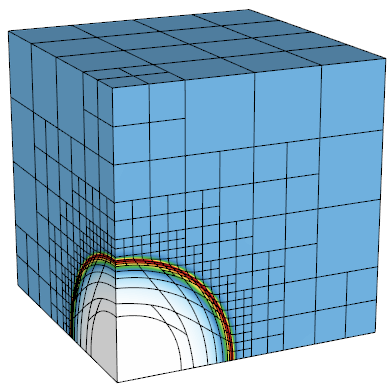
\includegraphics[width=0.3\textwidth]{figures/sedov-amr-900.png}
      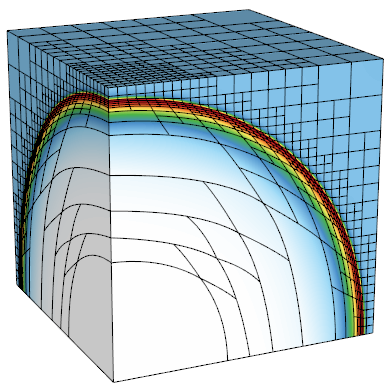
\includegraphics[width=0.3\textwidth]{figures/sedov-amr-2463.png} \\
      \small{Sedov AMR at steps 900 and 2463.} \\
      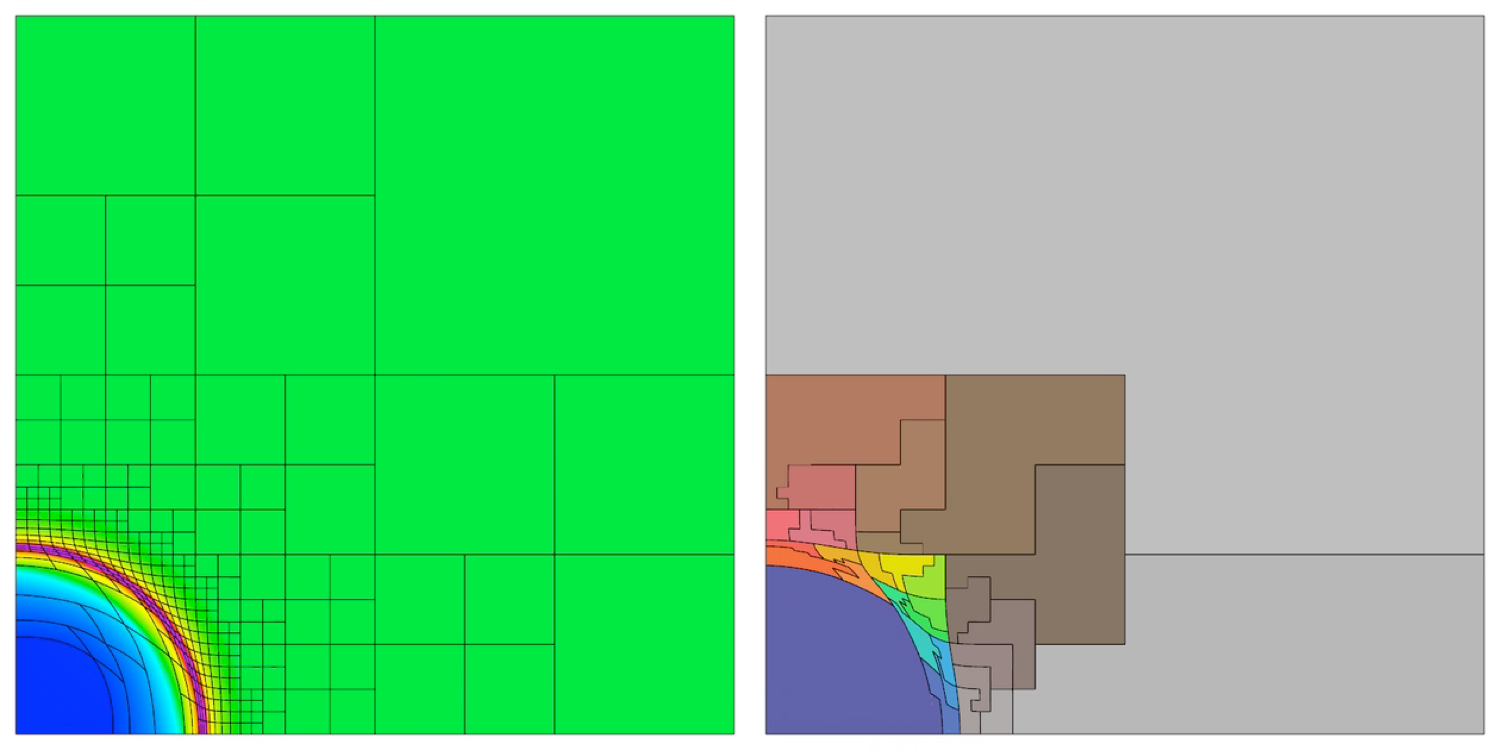
\includegraphics[width=0.9\textwidth]{{figures/sedov_animation_t8.19}.jpg} \\
      \small{Sedov AMR mesh (left) and partition (right) with space filling curves.}
    \end{column}
  \end{columns}
\end{frame}

\begin{frame}
  \frametitle{MFEM Laghos MiniApp - Early Sierra Results (T. Kolev, V. Tomov)}
  \begin{columns}
    \begin{column}{0.5\textwidth}
      \begin{itemize}
        \item 3rd order velocity and position (continuous kinematic), 2nd order internal
          energy (discontinuous thermodynamic) finite elements (Q3Q2)
        \item Mesh vertex repositioning without AMR
        \item Four GPUs/node with one MPI process/GPU
        \item More than 256K (256*1000) elements ('zones') required for
          scaling to ~30 GPUs, 16M elements required for 1024 GPUs
      \end{itemize}
    \end{column}
    \begin{column}{0.5\textwidth}
      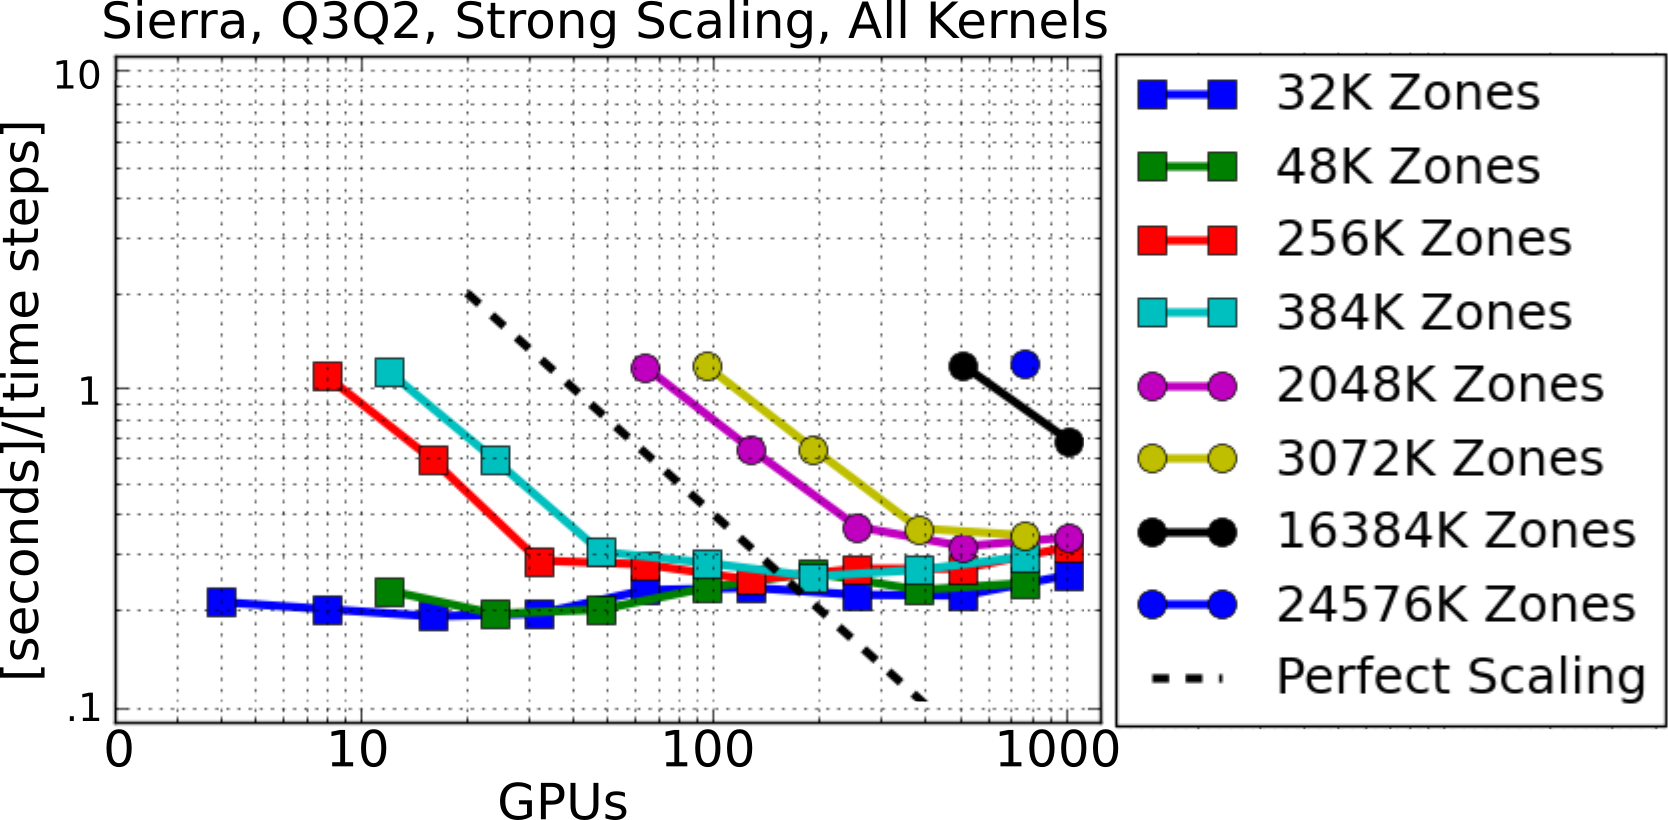
\includegraphics[width=\textwidth]{figures/laghos_strong_Q3Q2_sierra_cws.png} \\
      \small{Strong scaling for Laghos on Sierra of pure CUDA version.
      A zone is a mesh element.}
    \end{column}
  \end{columns}
\end{frame}

\begin{frame}
  \frametitle{MFEM Laghos MiniApp - Next Steps for Load Balancing}
  Task Mapping
  \begin{itemize}
    \item Ensure proceses that are assigned to the same node share domain data
    \item Zoltan2 (Karen Devine, SNL) geometric methods support the mapping of
      the network partition to the domain partition
  \end{itemize}
  EnGPar
  \begin{itemize}
    \item Integrate EnGPar w/MFEM
    \item Predictive balancing prior to mesh adaptation to (1) avoid memory 
      exhaustion and (2) create a post adaptation partition w/ acceptable imbalance
    \item Tune post adapt partition to (1) minimize induced communications between
      nodes and (2) reduce work imbalance
    \item Complete acceleration of critical EnGPar procedures - initial work
      completed with Kokkos
  \end{itemize}
\end{frame}

\begin{frame}
  \frametitle{}
  \center \huge{Balancing Finite Volume CFD}
\end{frame}

\begin{frame}
  \frametitle{FUN3D - Finite Volume CFD}
  Eric Nielsen and Aaron Walden at NASA Langley \\
  Summit ESP: ``Enabling Human Exploration of the Red Planet''
  \begin{columns}
    \begin{column}{0.5\textwidth}
      Goals
      \begin{itemize}
        \item Science: Better understanding of retropropulsion flow physics during Mars entry of human-scale lander
        \item Computational: Demonstrate production readiness and efficiency advantages of GPU implementation at scale
      \end{itemize}
    \end{column}
    \begin{column}{0.5\textwidth}
      \begin{figure}
        \centering
        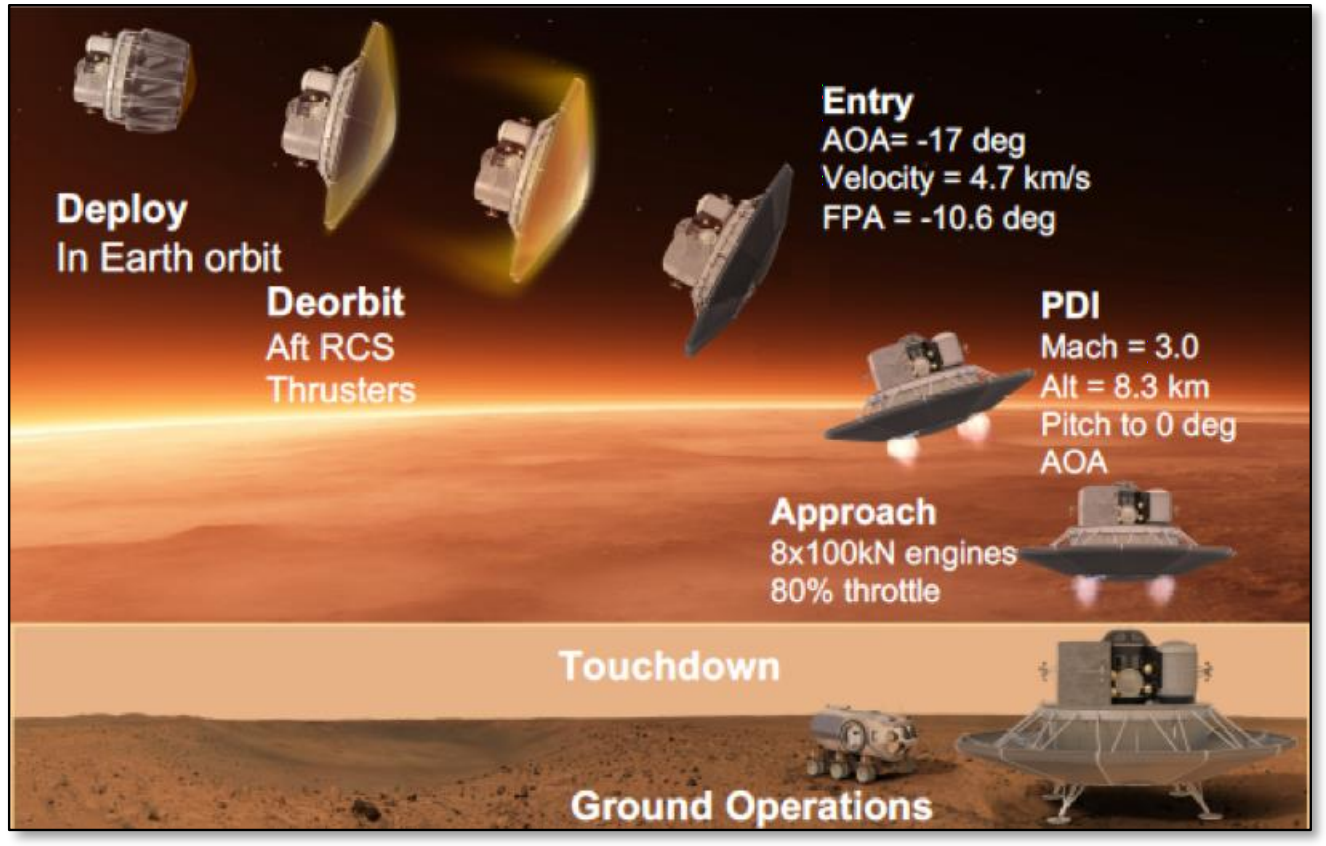
\includegraphics[width=.9\textwidth]{figures/fun3d-EDL.png}
      \end{figure}
    \end{column}
  \end{columns}
\end{frame}

\begin{frame}
  \frametitle{FUN3D - Early Summit Results (E. Nielsen and A. Walden)}
  \begin{columns}
    \begin{column}{0.5\textwidth}
      Partitioning Approach
      \begin{itemize}
        \item ParMETIS: mesh vertices $\rightarrow$ graph nodes,
          mesh edges $\rightarrow$ graph edges
        \item Mesh vertices hold DOFs
        \item EnGPar is integrated and being tested
      \end{itemize}
      Weak Scaling - nearly linear
      \begin{itemize}
        \item 13.2B (13.2*10$^9$) vertices, 58B elements, at 1024 nodes.
        \item GPU: MPI+CUDA, 3 ranks/socket, MPI via GPUDirect
        \item CPU: MPI+OpenMP, ranks/socket, 168 threads per node (SMT4)
      \end{itemize}
      GPU node-level performance is 23-37 times faster at scale than CPUs
    \end{column}
    \begin{column}{0.5\textwidth}
      \begin{figure}
        \centering
        Weak Scaling \\
        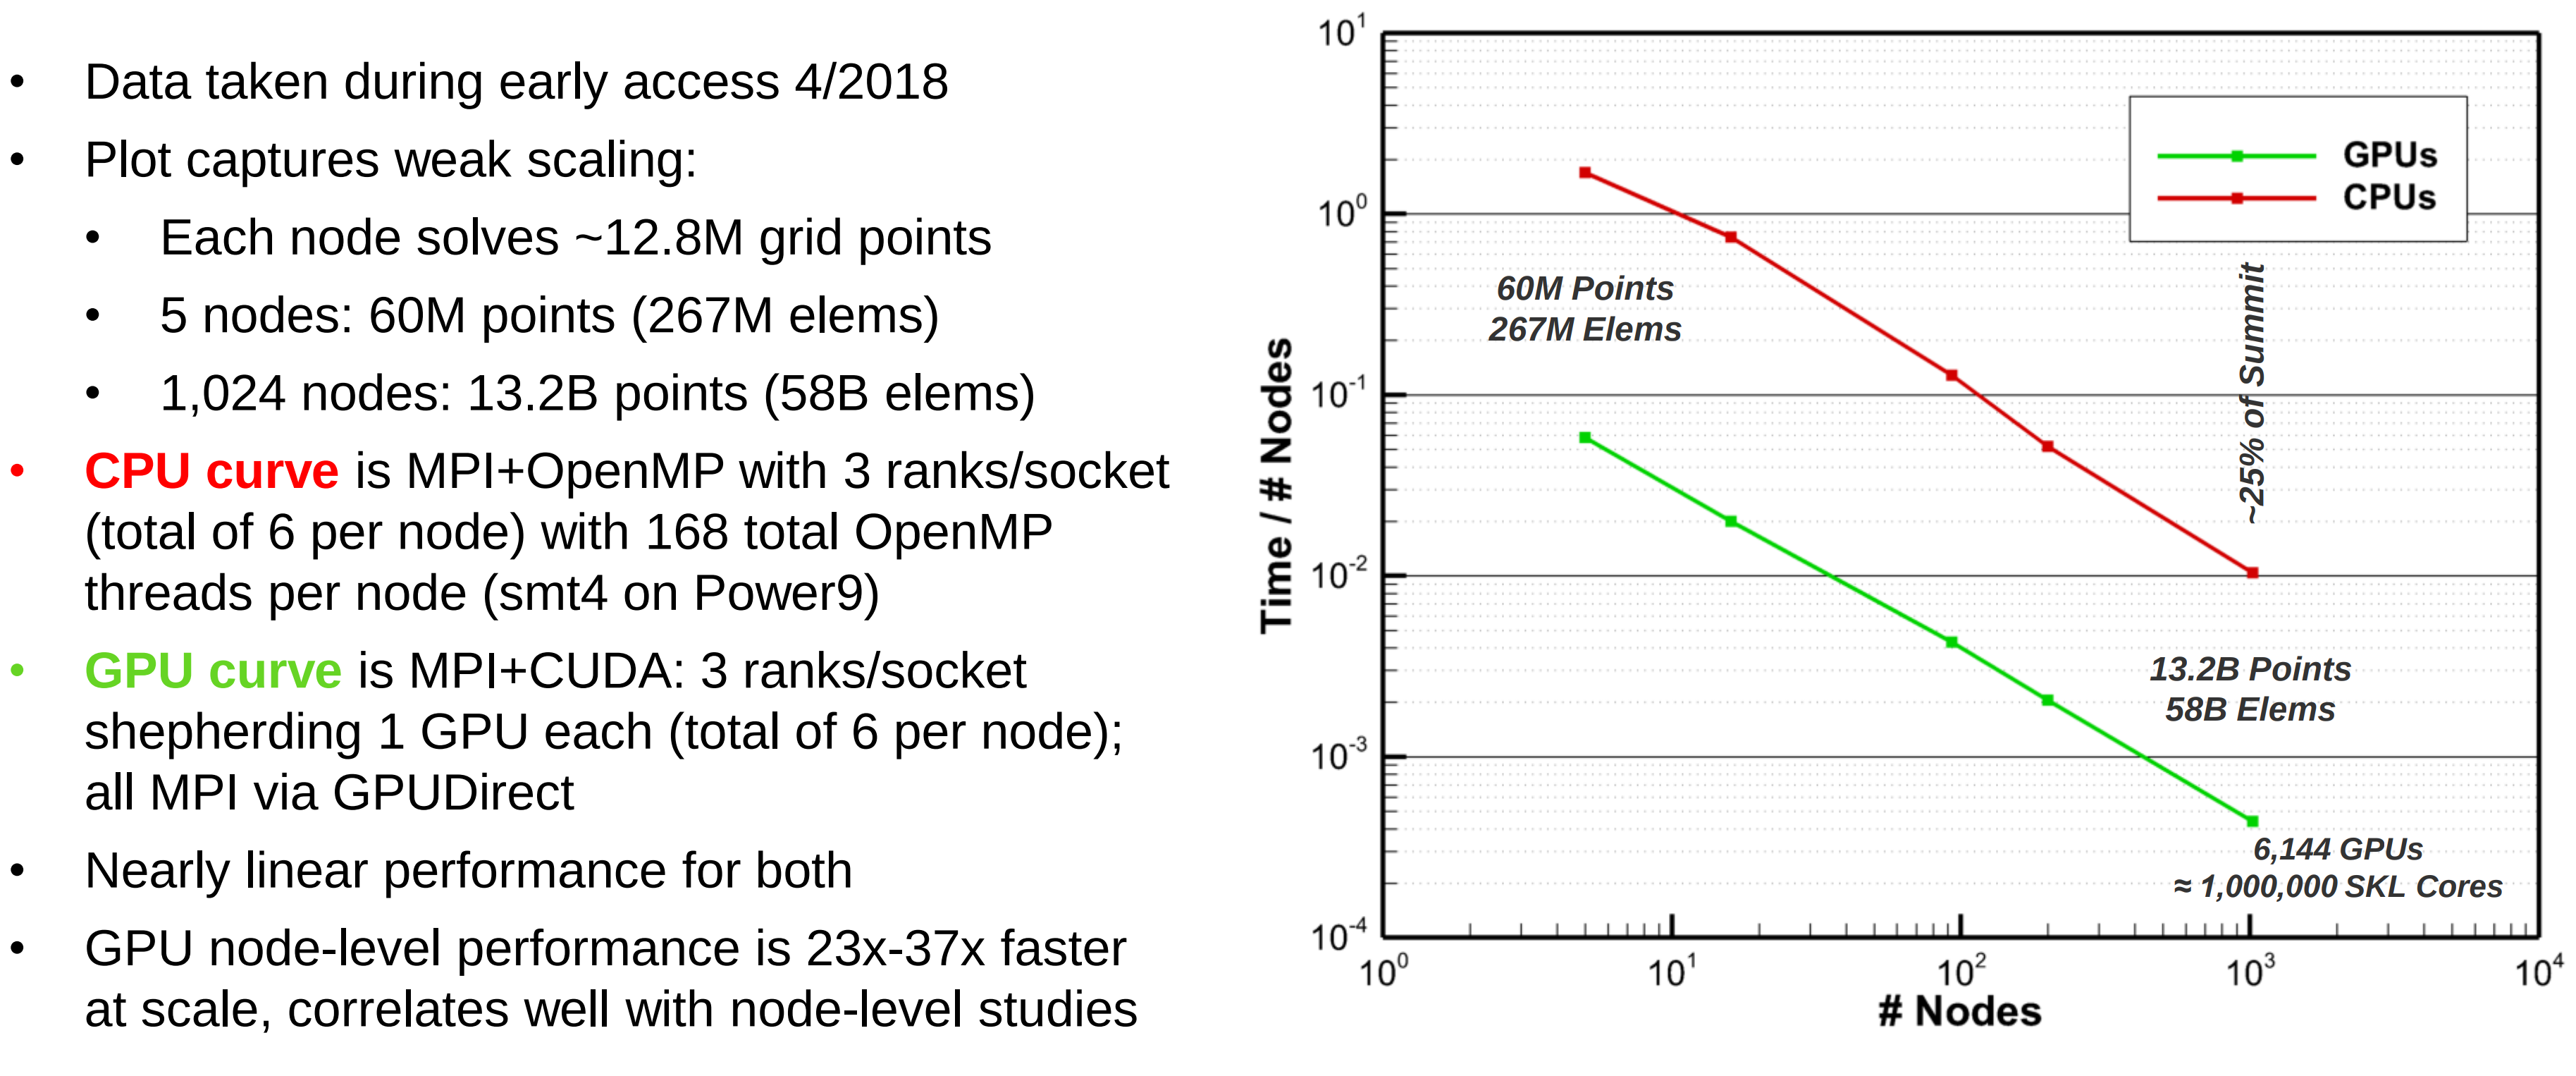
\includegraphics[width=\textwidth]{figures/fun3d-summit.png}
      \end{figure}
    \end{column}
  \end{columns}
\end{frame}

\begin{frame}
  \frametitle{}
  \center \huge{Balancing Unstructured Mesh Particle-in-Cell}
\end{frame}

\begin{frame}
  \frametitle{XGC - Fusion Plasma Physics}
  CS Chang, Princeton Plasma Physics Laboratory \\
  Summit ESP: ``Using XGC to predict ITER’s boundary plasma performance and its impact on fusion efficiency''
  \begin{columns}
    \begin{column}{0.5\textwidth}
      Goals
      \begin{itemize}
        \item Science: Study tokamak plasma performance near boundary
	\item Computational: Develop platform for multiscale plasma physics simulations on leadership systems
      \end{itemize}
    \end{column}
    \begin{column}{0.5\textwidth}
      \begin{figure}
        \centering
        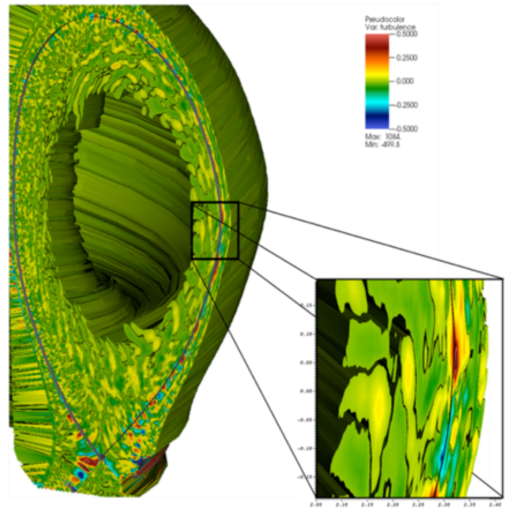
\includegraphics[width=.7\textwidth]{figures/xgcCase.png} \\
        \tiny{DIII-D Geometry: Boundary turbulence saturates
        in $<$ 0.1ms, core turbulence in a few ms.}
      \end{figure}
    \end{column}
  \end{columns}
\end{frame}

\begin{frame}
  \frametitle{XGC - Partitioning Approach (CS Chang)}
  \begin{columns}
    \begin{column}{0.5\textwidth}
      %https://scorec.rpi.edu/~shephard/some%20fusion%20stuff/xgc-book-chapter.pdf
      %https://cug.org/proceedings/cug2016_proceedings/includes/files/pap178s2-file2.pdf
      \begin{itemize}
        \item Each process has entire copy of 2D poloidal mesh, mesh repeated N
          times in the toroidal direction
        \item Radial 1D partition of poloidal mesh vertices used for push and collision
        \item Each plane has a set of processes working on it, each process is
          assigned a different part
        \item Particles are owned by the part/process they reside in
        \item Load balancer monitors wall clock time of push and collision steps
          and uses a Golden Section Search to minimize the time as a function of
          the max particle count per process
      \end{itemize}
    \end{column}
    \begin{column}{0.5\textwidth}
      \begin{figure}
        \centering
        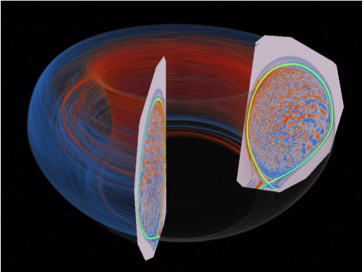
\includegraphics[width=.5\textwidth]{figures/xgcTokamakSimulation.png} \\
        \small{3D tokamak simulation.  2 poloidal planes shown.}
        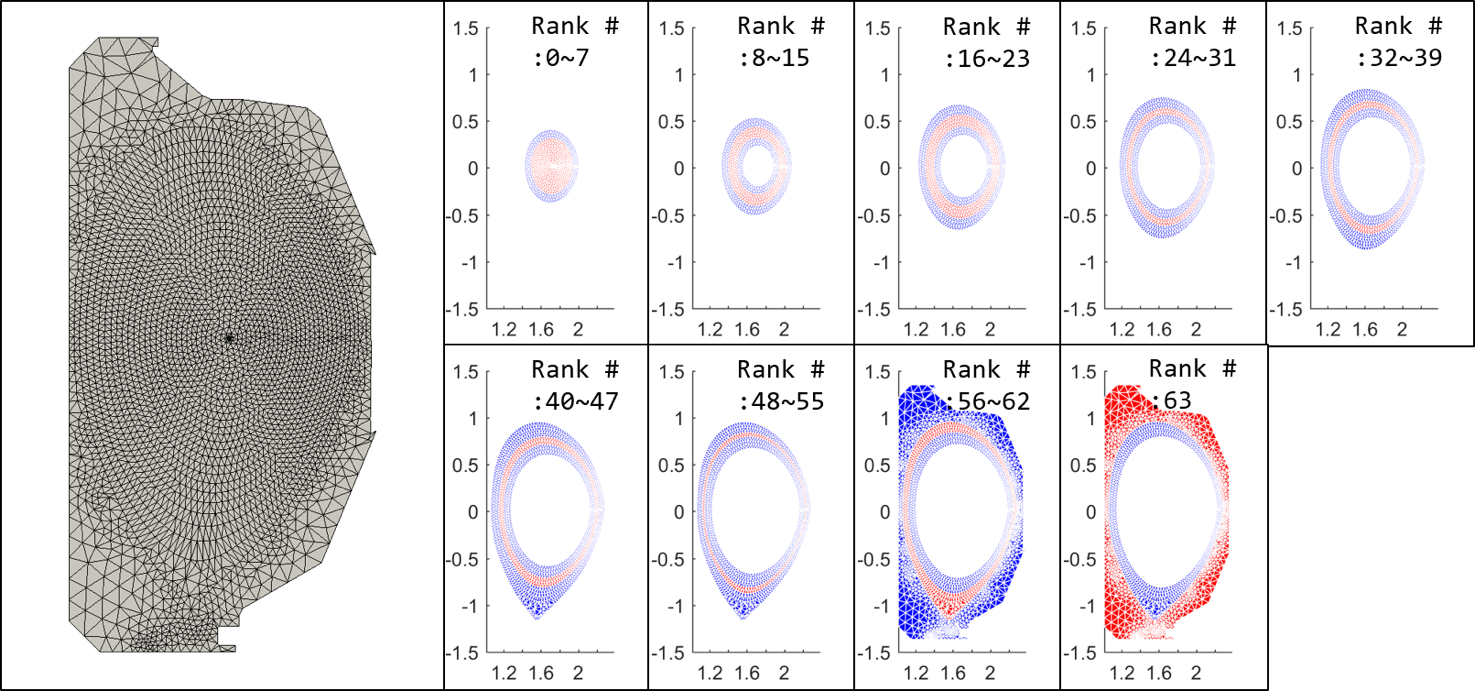
\includegraphics[width=.85\textwidth]{figures/xgcMeshDistribution.png} \\
        \small{2D mesh and process groups.}
      \end{figure}
    \end{column}
  \end{columns}
\end{frame}

\begin{frame}
  \frametitle{XGC - Early Summit Results (CS Chang)}
  \begin{columns}
    \begin{column}{0.3\textwidth}
      Strong Scaling vs Titan
      \begin{itemize}
        \item Scaling runs using up to 44\% of Summit, 2048 nodes
        \item MPI + CUDA (electron push) + OpenACC (collision) + OpenMP
        \item 25 times faster than Titan % HERE
      \end{itemize}
      CPU+GPU performance is 11 times faster than CPU only at 12,288 GPUs (2Ki
      nodes)
    \end{column}
    \begin{column}{0.65\textwidth}
      \begin{figure}
        \centering
        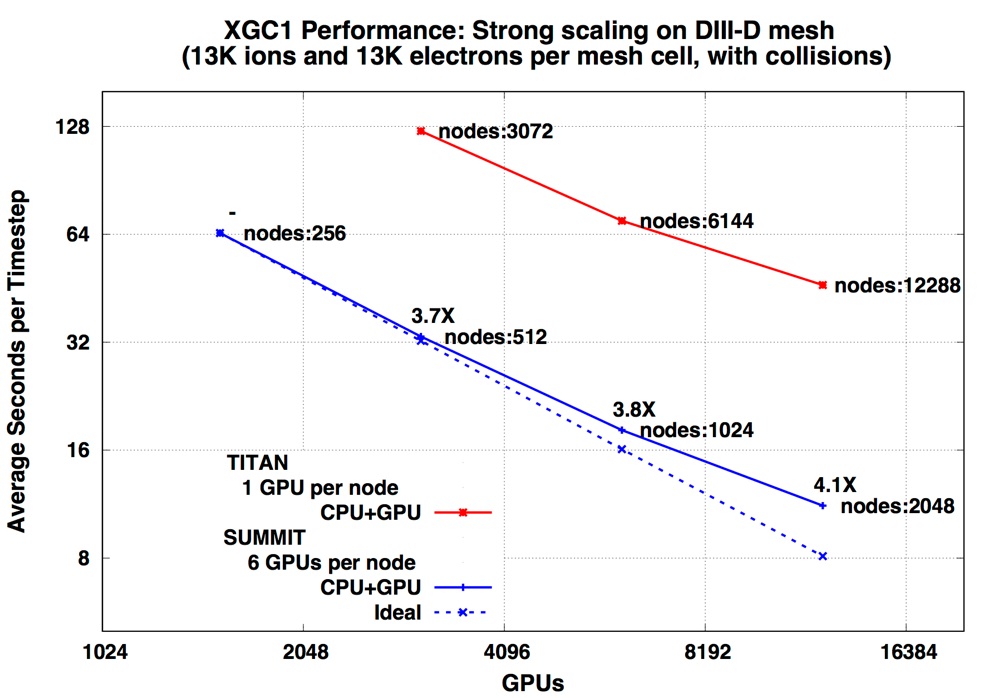
\includegraphics[width=\textwidth]{figures/xgcStrongScaling.png}
      \end{figure}
    \end{column}
  \end{columns}
\end{frame}

\begin{frame}
  \frametitle{XGC - Ongoing Developments}
  \begin{columns}
    \begin{column}{0.5\textwidth}
      Developing tools for unstructured mesh PIC
      \begin{itemize}
        \item Distributed mesh with `safe' zones to avoid communication during
          push
        \item Bulk communication protocol that accounts for `safe' zones and can
          quickly update field data already on the GPU - Omega\_h [1] for GPU mesh
        \item Particle load balancing with EnGPar
        \begin{itemize}
          \item Construct subgraphs connecting processes
            for each overlapping safe zone.
          \item Set the weights of vertices to be the
            number of particles
in the elements for
            the overlapping safe zone.
          \item Diffusively migrate weight (\# of particles) in each
            subgraph until processes are balanced.
        \end{itemize}
      \end{itemize}
      {\tiny [1] \url{github.com/SNLcomputation/omega_h} }
    \end{column}
    \begin{column}{0.5\textwidth}
      \begin{figure}
        \centering
        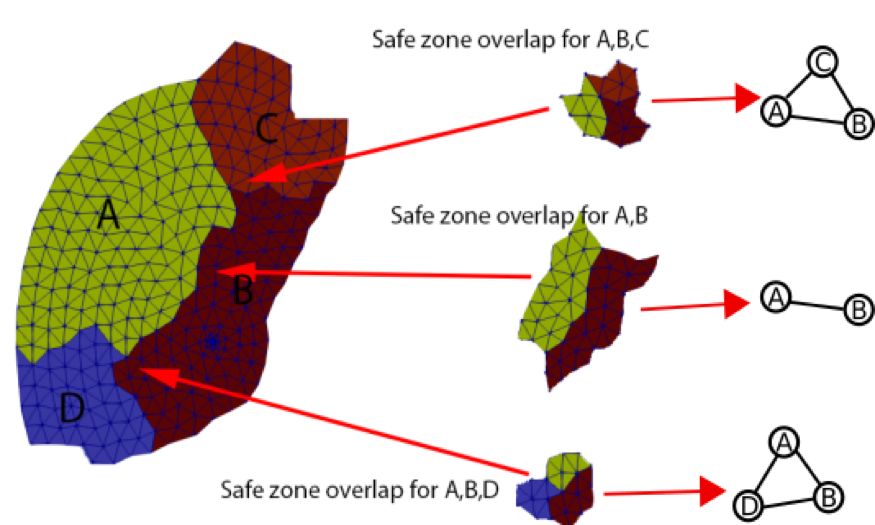
\includegraphics[width=.6\textwidth]{figures/engparPIC.png}\\
        \small{Subgraphs created from core parts and safe zone parts.}
      \end{figure}
    \end{column}
  \end{columns}
\end{frame}

\begin{frame}
  \frametitle{Closing Remarks}
  Summit GPUs provide $>$90\% of the system performance
  \begin{itemize}
    \item Technically heterogeneous...
    \item Cost to thread, optimize and load balance for the CPUs is not worth
      the person-hours
  \end{itemize}
  Focus on providing a `decent' load imbalance to GPUs with minimized induced inter-GPU data movement
  \begin{itemize}
    \item Placing processes near those they share domain data with
    \item Optimizing partitions for communication, possibly sacrificing load balance
    \item Predictively load balance to reduce calls to balancer
  \end{itemize}
  Many more challenges if we had a processor/node with multiple specialized accelerators
  (e.g., compression, fft, spmv, graph traversal, encryption, etc...)
  \begin{itemize}
    \item Will current programming models/tools work effectively? Major code rewrite?
    \item Many post exascale technologies in the pipeline:
      \url{www.crnch.gatech.edu/sites/default/files/02-siamcse-2019-shalf.pdf}
  \end{itemize}
\end{frame}

\begin{frame}
  \begin{center}
    {\huge
      Thank You\\
      \bigskip
      \bigskip
      \bigskip
      \bigskip
      \bigskip
      \huge
      Questions?\\
      \bigskip
      \bigskip
      \bigskip
    }
  \end{center}
  \large
  Acknowledgements:\\
  \begin{itemize}
    \item NSF SI2-SSE: Fast Dynamic Load Balancing Tools for Extreme Scale Systems
    \item DOE FASTMath SCIDAC Institute
    \item CEED ECP
  \end{itemize}
\end{frame}

\end{document}
